\documentclass[a4paper,12pt]{article}

\def\term{Fall}
\def\year{2024}
\def\lecturer{Huang} %Wei-Cheng Huang
\def\coursenumber{Math265}
\def\coursename{Real Analysis}

\makeatletter
\ifx \nauthor\undefined
  \def\nauthor{Kaifeng Lu}
\else
\fi

\makeatletter
\ifx \email\undefined
  \def\email{\href{klu15@u.rochester.edu}{klu15 at u dot rochester dot edu}}
\else
\fi

\title{\coursenumber \, \coursename \, Class Notes}
\author{Based on lectures by Prof. \lecturer \\\small Notes taken by \nauthor\\\small Errata: \,\email}
\date{\term\ \year}

\usepackage{amsmath}
\usepackage{amsfonts}
\usepackage{amssymb}
\usepackage{amsthm}
\usepackage{caption}
\usepackage{enumitem}
\usepackage{fancyhdr}
\usepackage[margin=1in]{geometry}
\usepackage{listings}
\usepackage{multicol,multirow}
\usepackage[hidelinks]{hyperref}
\usepackage{parskip}
\usepackage{tikz}
\usepackage{wrapfig}
\usepackage{mathtools}
\usepackage{caption}
\usepackage{subcaption}

% Theorems-renew
\theoremstyle{definition}
\newtheorem*{aim}{Aim}
\newtheorem*{axiom}{Axiom}
\newtheorem*{claim}{Claim}
\newtheorem*{corollary}{Corollary}
\newtheorem*{conjecture}{Conjecture}
\newtheorem*{definition}{Definition}
\newtheorem*{example}{Example}
\newtheorem*{exercise}{Exercise}
\newtheorem*{fact}{Fact}
\newtheorem*{law}{Law}
\newtheorem*{lemma}{Lemma}
\newtheorem*{notation}{Notation}
\newtheorem*{proposition}{Proposition}
\newtheorem*{question}{Question}
\newtheorem*{theorem}{Theorem}
\newtheorem*{assumption}{Assumption}

\newtheorem*{remark}{Remark}
\newtheorem*{warning}{Warning}

% Special sets
\newcommand{\C}{\mathbb{C}}
\newcommand{\N}{\mathbb{N}}
\newcommand{\Q}{\mathbb{Q}}
\newcommand{\R}{\mathbb{R}}
\newcommand{\Z}{\mathbb{Z}}
\newcommand{\F}{\mathbb{F}}
\newcommand{\neighbor}[2]{V_{#1}{(#2)}}

% Brackets
\newcommand{\abs}[1]{\left\lvert #1\right\rvert}
\newcommand{\norm}[1]{\left\lVert #1\right\rVert}
\newcommand{\highlight}[1]{\textit{\textbf{\underbar{#1}}}}
\newcommand{\bra}{\langle}
\newcommand{\ket}{\rangle}

%Sequence
\newcommand{\seq}[2]{(#1_{#2})}
\newcommand{\seqfun}[2][n]{(f_{#1}(#2))}

%Abbv
\newcommand{\st}{\text{ s.t. }}
\newcommand{\limx}[2]{\lim_{x\rightarrow #1} {#2}}
\newcommand{\limn}[1]{\lim_{n\rightarrow\infty} {#1}}
\newcommand{\ds}{\displaystyle}

%RenewCommand
\renewcommand\qedsymbol{$\blacksquare$}

\hypersetup{
    colorlinks,
    citecolor=black,
    filecolor=black,
    linkcolor=black,
    urlcolor=black,
    pdfpagemode=FullScreen
}

%Figures
\newcommand{\sidefig}[2]{
  \begin{wrapfigure}{#1}{1.7\textwidth}
    \includegraphics[width=0.6\textwidth]{image/#2}
    \centering
  \end{wrapfigure}
}
\newcommand{\centerfig}[2][0.6]{
  \begin{figure}[h]
    \includegraphics[width=#1 \textwidth]{image/#2}
    \centering
  \end{figure}
}



%%%%%%%%%%%%%%%%%%%%%%
% Set up fancy header/footer
\pagestyle{fancy}
\fancyhead[LO,L]{\nauthor}
\fancyhead[CO,C]{\coursenumber \ - Lecture notes}
\fancyhead[RO,R]{Prof. \lecturer}
\fancyfoot[LO,L]{}
\fancyfoot[CO,C]{\thepage}
\fancyfoot[RO,R]{}
\renewcommand{\headrulewidth}{0.4pt}
\renewcommand{\footrulewidth}{0.4pt}
%%%%%%%%%%%%%%%%%%%%%%

\begin{document}
\maketitle
\centerfig{cover.jpg}
\newpage

\section{Preliminaries}
Still working on it...(missed 1st month due to late enrollment)
% \newpage

% \subsection{Sets and Functions}

% \newpage

% \subsection{Mathematical Induction}

% \newpage

% \subsection{Finite and Infinite Sets}

% \newpage

\section{The Real Numbers}
Still working on it...
% \newpage

% \subsection{The Algebraic and Order Properties of $\R$}

% \newpage

% \subsection{Absolute Value and the Real Line}

% \newpage

% \subsection{The Completeness Property of $\R$}


% \newpage

% \subsection{Applications of Supremum}

% \newpage
% \subsection{Intervals}

\newpage
\section{Sequences and Series}
\subsection{Sequences and their limits}

\begin{definition}[\textbf{Sequence}]
    A \highlight{sequence of real numbers} is a \textit{function} from $\N$ to $\R$.
\end{definition}


We adopt the notation with a \textit{sequence}:
\[\,a:\N\rightarrow\R\]
where instead of writing \(a(1), a(2), \dots\), we write it as \(a_1, a_2, \dots\) which we called them 
\highlight{terms} or \highlight{elements} of the sequence.\\

\begin{notation}

\[(a_n)_{n=1}^\infty  \text{ or }  (a_n)_{n\in\N}  \text{ or }  (a_n)  \text{ or }  (a_n|n\in \N)\]\\
\end{notation}

\begin{definition}[\textbf{Converge to x}]
    A sequence \((x_n)\in\R\) \highlight{converges} to \(x\in\R\) if 
    \[\forall \varepsilon >0,\, \exists N_\varepsilon \in \N \text{ such that }n\ge N_\varepsilon \rightarrow\abs{x_n - x} <\varepsilon\]
    We write \[\lim_{n\to\infty}x_n = \lim_{n\to\infty}(x_n) = x.\]\\
\end{definition}

\begin{definition}[\textbf{Convergent \& Divergent}]
    A sequence is \highlight{convergent} if it has a \highlight{limit} in \(\R\), and is \highlight{divergent} if it 
    has \highlight{no limit} in $\R$.\\
\end{definition}

\newpage
\begin{theorem}[\textbf{Uniqueness of Limit}]
    A sequence in $\R$ can have \highlight{at most one} limit. Or, the limit of a sequence is \highlight{unique} if the limit exists 
\end{theorem}
\begin{proof}
    Let \((x_n)\) be a sequence of real numbers. Suppose \(x,x'\) are limits of \((x_n)\). We want to prove \(x = x'\) by contradiction.
    \\\\Assume \(\abs{x-x'} > 0\). If we consider \(\varepsilon := \frac{1}{3}\abs{x-x'}>0\), then\\
    \indent \(\text{The existence of } \lim_{x_n \to x}\text{implies that } \exists N_1 \in \N \text{ such that } \abs{x_n-x} < \varepsilon\text{ if }n\ge \N_1. \)\\
    \indent \(\text{Similarly, existence of } \lim_{x_n \to x'} \text{implies that } \exists N_2 \in \N \text{ such that } \abs{x_n-x'} < \varepsilon\text{ if }n\ge \N_2. \)\\
    Thus,
    \begin{align*}
        \abs{x-x'} & \le \abs{x-x_{N_1+N_2}+x_{N_1+N_2}-x'} & \\
                   & \le \abs{x-x_{N_1+N_2}}+\abs{x_{N_1+N_2}-x'} \text{ by triangle inequality}\\
                   & < \varepsilon+\varepsilon \\
                   & = \frac{2}{3}\abs{x-x'}
    \end{align*}
    Then, 
    \[\frac{1}{3}\abs{x-x'}<0,\text{which is a contradiction}\]
    we thereby prove by contradiction that
    \[\abs{x-x'} = 0\text{, which is equivalent to } x=x'\]
\end{proof}

\begin{example}
    \[\lim_{n\to \infty}(\frac{1}{n}) = 0\]
    Goal: \(\forall \varepsilon>0,\) want to find \(N_\varepsilon\) such that \(\abs{\frac{1}{n}-0} < \varepsilon\) for \(n>N\), 
    so it suffices to show that \\
    \[\frac{1}{n}<\varepsilon \Leftrightarrow \frac{1}{\varepsilon} < n\]
\end{example}

\begin{proof}
    Let \(\varepsilon>0\). Apply Archimedean's property to \(\frac{1}{\varepsilon}\), then
    \begin{align*}
        & \exists N\in \N \text{ such that }\frac{1}{\varepsilon}<N \\
        \Rightarrow & \forall n \ge N, \abs{\frac{1}{n}-0} = \frac{1}{n}\le \frac{1}{N} < \varepsilon.\\
        \Rightarrow & \lim_{n \to \infty}\frac{1}{n} = 0
    \end{align*}
\end{proof}
\newpage
\begin{theorem}
    Let \((x_n)\) be a sequence of real numbers, and let \(x \in \R\). The following are equivalent:
\begin{enumerate}
    \item \(x_n \rightarrow x\)
    \item \(\forall \varepsilon > 0, \exists N \in \N \text{ such that } \abs{x_n-x}<\varepsilon,\text{ for }n\ge \N \)
    \item \(\dots \dots x - \varepsilon<x_n<x+\varepsilon\dots\dots\)
    \item \(\forall\varepsilon\text{-neighborhood } V_\varepsilon(x),\exists N \in \N \text{ such that } x_n \in V_\varepsilon(x) \text{ for } n\ge N\)\\
\end{enumerate}
\highlight{Sketch of proof:}
\[(1)\Leftrightarrow(2)\Leftrightarrow(3)\Leftrightarrow(4)\]
\end{theorem}

\begin{proposition}
    \[\lim_{n\to \infty}(2\sqrt{2n+1}-\sqrt{2n})=0\]
\end{proposition}

\begin{proof}
    Let \(\varepsilon > 0\). Consider \[N = \lceil\frac{1}{2}(\frac{1}{2\varepsilon})^2\rceil\in\N\]
    \[n>N\Rightarrow n>\frac{1}{2}(\frac{1}{2\varepsilon})^2 \Rightarrow \frac{1}{2\sqrt{2n}}<\varepsilon\Rightarrow\abs{\sqrt{2n+1}-\sqrt{2n}} = \dots = \frac{1}{\sqrt{2n+1}+\sqrt{2n}}<\varepsilon\]
\end{proof}

\begin{remark}
    \[\lim_{n\to\infty}(-1)^n\text{ does not exist.}\]\\
\end{remark}

\begin{definition}[\textbf{m-tail}]
    If \((x_n)\) is a sequence of real numbers and \(m \in \N\), then the \highlight{m-tail} of \((x_n)\) is the sequence 
    \[\{x_{n+m}:n\in\N\}=\{x_{m+1}, x_{m+2}, \dots\}\]
\end{definition}

\begin{theorem}
    Let \((x_n)\) be a sequence and \(m\in\N\). Then \((x_n)\) is \highlight{convergent} iff \((x_{n+m})\) is \highlight{convergent}. 
    Moreover,\[\lim_{n\to\N}(x_n) = \lim_{n\to\N}(x_{n+m})\]
\end{theorem}

\begin{proof}
    \((\Rightarrow)\)\\
    Suppose \(x_n\to x\). Let\[\varepsilon>0, \exists N_\varepsilon >0, \text{ such that } \abs{x_n-x}<\varepsilon \text{ for }n\ge N_\varepsilon\]
    Consider \({N_\varepsilon}':=N_\varepsilon + m\) then
    \[n+m \ge {N_\varepsilon}' \Rightarrow n\ge N_\varepsilon \Rightarrow n+m\ge N_\varepsilon \Rightarrow \abs{x_{n+m}-x}<\varepsilon\]
    It follows that \[n\ge N_\varepsilon \Rightarrow n+m \ge N_\varepsilon \Rightarrow \abs{x_{n+m}-x}<\varepsilon\]
    \newpage
    \((\Leftarrow)\)\\
    Suppose \(x_{n+m}\rightarrow x\).
    \[\forall \varepsilon>0,\exists N_\varepsilon>0 \text{ such that } \abs{x_{n+m}<\varepsilon}, \forall n\ge N_\varepsilon\]
    Consider \(N:=N_\varepsilon+m\). Then 
    \begin{align*}
        & n\ge N = N_\varepsilon+m \\
        & \Rightarrow n-m \ge N_\varepsilon \\
        & \Rightarrow\abs{x_{(n-m)+m}-x}<\varepsilon \\
        & \Rightarrow\abs{x_n-x}<\varepsilon
    \end{align*}
\end{proof}

\begin{remark}
    We say that a sequence \((x_n)\) \highlight{ultimately} has a property if that property holds for some tail of \((x_n)\)\\
\end{remark}

\begin{theorem}
    Let \(x_n\) be a sequence of real numbers. 
    Let \(a_n\) be a sequence of positive real numbers such that \(\lim_{n\to \infty}a_n=0\).
    If \(\exists c>0, m\in \N, x\in \R\) such that \[\abs{x_n-x} \le c\cdot a_n,\forall n\ge m\]
    then \[x_n\to x\]
\end{theorem}

\begin{proof}
    We know that
    \[\forall \varepsilon>0, \exists N\ge 0\text{ s.t. } \abs{a_n}<\frac{\varepsilon}{c},\, \forall n\ge N\]
    Consider \(N'=max\{N,m\}, \forall n\ge N'\). Then 
    \[\abs{x_n-x}\le Ca_n = c\abs{a_n}<c\cdot\frac{\varepsilon}{c} = \varepsilon\]
    \[\Rightarrow x_n\rightarrow x\]
\end{proof}

\begin{proposition}
    \[\lim_{n\to\infty}\frac{17}{2+3n}=0\]
    \begin{proof}
        \[\abs{\frac{17}{2+3n}-0} = \frac{17}{2+3n} \le \frac{13}{3n} = \frac{17}{3}\cdot\frac{1}{n}\]
        Apply the theorem above with \[a_n=\frac{1}{n},c = \frac{17}{3}, m=1\]
        \[\Rightarrow\lim_{n\to\infty}\frac{17}{2+3n}=0\text{, since }\lim_{n\to\infty}\frac{1}{n}=0\]
    \end{proof}
\end{proposition}

\newpage
\begin{proposition}
    \[\forall c>0, \lim_{n\to\infty}c^{\frac{1}{n}}=1\]
    \begin{proof}

        \highlight{Case 1: c = 1} \[\lim_{n\to\infty}c^{\frac{1}{n}}=1\]
        \highlight{Case 2: c > 1}\\\\
        Let \(d_n = c^{\frac{1}{n}}-1\). Then \(\forall n, d_n>0\). It follows that 
        \begin{align*}
            (d_n+1)=c^{\frac{1}{n}} & \Rightarrow c= (1+d_n)^n\ge 1+n\cdot d_n\text{ by Bernoulli's inequality}\\
            & \Rightarrow d_n\le (c-1)\cdot \frac{1}{n} \\
            & \Rightarrow \abs{c^{\frac{1}{n}}-1} = d_n\le (c-1)\cdot\frac{1}{n}
        \end{align*}
        Apply the theorem with \[C = c-1,a_n = \frac{1}{n}, m=1,x=1\]
        \[\lim_{n\to\infty}c^{\frac{1}{n}}=1\]
        \highlight{Case 3: c < 1(Note that we cannot use Bernoulli inequality here)}\\\\
        Define \(e_n\) to be a sequence that satisfies \[c^{\frac{1}{n}} = \frac{1}{1+e_n}\]
        Then \(e_n>0\forall n\).
        \[c = \frac{1}{(1+e_n)^n}\le\frac{1}{1+n\cdot e_n} < \frac{1}{n\cdot e_n}\]
        \[\Rightarrow e_n < \frac{1}{c}\cdot \frac{1}{n}\]
        \[1-c^{\frac{1}{n}}= 1-\frac{1}{1+e_n}= \frac{e_n}{1+e_n}<e_n<\frac{1}{c}\cdot \frac{1}{n}\]
        Apply the theorem with \[a_n = \frac{1}{n}, m=1,C=\frac{1}{c}, x=1\]
        \[\lim_{n\to\infty} c^\frac{1}{n}=1\]
    \end{proof}
\end{proposition}

\newpage
\subsection{Limit Theorems}
\begin{definition}[\text{Bounded sequence}]
    A sequence \(\seq{x}{n}\in\R\) is \highlight{bounded} if
    \[\exists M>0 \st\forall n\in\N, \abs{x_n}\le M\]
\end{definition}

\begin{theorem}
    A convergent sequence \(\seq{x}{n}\in\R\) is bounded.

    \begin{center}
        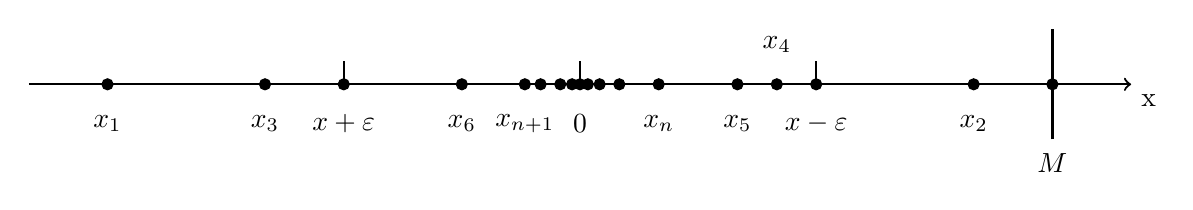
\begin{tikzpicture}
            \draw[thick,->] (-7,0) -- (7,0) node[anchor=north west] {x};
            \draw[thick] (0,0) -- (0,0.3);

            \filldraw[black] (-6,0) circle (2pt);
            \draw (-6,-0.5) node{\(x_1\)};
            \filldraw[black] (5,0) circle (2pt);
            \draw (5,-0.5) node{\(x_2\)};
            \filldraw[black] (-4,0) circle (2pt);
            \draw (-4,-0.5) node{\(x_3\)};
            \filldraw[black] (2.5,0) circle (2pt);
            \draw (2.5,0.5) node{\(x_4\)};
            \filldraw[black] (2,0) circle (2pt);
            \draw (2,-0.5) node{\(x_5\)};
            \filldraw[black] (-1.5,0) circle (2pt);
            \draw (-1.5,-0.5) node{\(x_6\)}; 
            \filldraw[black] (1,0) circle (2pt);
            \draw (1,-0.5) node{\(x_n\)}; 
            \filldraw[black] (-0.7,0) circle (2pt);
            \draw (-0.7,-0.5) node{\(x_{n+1}\)}; 
            \filldraw[black] (-0.5,0) circle (2pt);
            \filldraw[black] (-0.25,0) circle (2pt);
            \filldraw[black] (-0.1,0) circle (2pt);
            \filldraw[black] (0.5,0) circle (2pt);
            \filldraw[black] (0.25,0) circle (2pt);
            \filldraw[black] (0.1,0) circle (2pt);
            
            \filldraw[black] (0,0) circle (2pt);
            \draw (0,-0.5) node{0};
            
            \filldraw[black] (3,0) circle (2pt);
            \draw (3,-0.5) node{\(x-\varepsilon\)};
            \draw[thick] (3,0) -- (3,0.3);

            \filldraw[black] (-3,0) circle (2pt);
            \draw (-3,-0.5) node{\(x+\varepsilon\)};
            \draw[thick] (-3,0) -- (-3,0.3);

            \filldraw[black] (6,0) circle (2pt);
            \draw (6,-1) node{\(M\)};
            \draw[thick] (6,-0.7) -- (6,0.7);
        \end{tikzpicture}
    \end{center}

    \begin{proof}
        By definition of convergent sequence, let \(\varepsilon=1\):
        \[\exists N>0\st\forall n\ge N, \abs{x_n-x}<1\]
        Thus we have
        \begin{align*}
            &&-1&<x_n-x<1\\
            &\Rightarrow& -1+x&<x_n<x+1, \,\forall n\ge N
        \end{align*}
        Then define 
        \[M:=\max{\{\abs{x_1},\abs{x_2},\abs{x_3},\dots,\abs{-1+x},\abs{x+1}\}}\]
        \[\abs{x_n}\le M\]
    \end{proof}

    \begin{remark}
        By contrapositive, an unbounded sequence is divergent.\\
    \end{remark}
\end{theorem}

\begin{definition}
    Given sequence \(\seq{x}{n}, \seq{y}{n}\in\R\),
    we define following operations of sequence:
    \begin{itemize}
        \item \highlight{Sum} \((x_n+y_n)\)
        \item \highlight{Difference} \((x_n-y_n)\)
        \item \highlight{Product} \((x_n\cdot y_n)\)
        \item \highlight{Quotient} \((\frac{x_n}{y_n})\) if \(\forall n\in\N, y_n\neq 0\)
        \item \highlight{Multiple} \((c\cdot x_n)\)\\
    \end{itemize}
\end{definition}

\begin{theorem}[\textbf{Limit Laws}]
    Let \(\seq{x}{n}, \seq{y}{n}\in\R\) be sequences of real numbers with \(x_n\rightarrow x, y_n\rightarrow y\), 
    and let \(c\in\R\).
    Then
    \begin{itemize}
        \item \(x_n+y_n\rightarrow x+y\)
        \item \(x_n-y_n\rightarrow x-y\)
        \item \(x_n\cdot y_n\rightarrow x\cdot y\)
        \item \(c\cdot x_n\rightarrow c\cdot x\)
        \item If \(\forall n\in\N, y_n\neq 0\) and \(y\neq 0\), then \(\frac{x_n}{y_n}\rightarrow \frac{x}{y}\)
    \end{itemize}

    \newpage
    \begin{proof}[Proof of Sum]:

        \(\forall \varepsilon>0\),
        \[\exists N_1\in\N \st \forall n\ge N_1, \abs{x_n-x}<\frac{\varepsilon}{2}\]
        \[\exists N_2\in\N \st \forall n\ge N_2, \abs{y_n-y}<\frac{\varepsilon}{2}\]
        Consider \[N:=\max{\{N_1,N_2\}}\]
        Then
        \begin{align*}
            \forall n\ge N, &\abs{(x_n+y_n)-(x+y)}\\
            =&\abs{x_n-x+y_n-y}\\
            \le& \abs{x_n-x}+\abs{y_n-y}\\
            =&\frac{\varepsilon}{2}+\frac{\varepsilon}{2}\\
            =&\varepsilon
        \end{align*}
    \end{proof}

    \begin{proof}[Proof of Difference]:

        Similarly,
        \begin{align*}
            \forall n\ge N, &\abs{(x_n-y_n)-(x-y)}\\
            \le& \abs{x_n-x}+\abs{y_n-y}
        \end{align*}
    \end{proof}

    \begin{proof}[Proof of Product]:
        Since \(\seq{x}{n}\) is convergent, it is also bounded. Thus,
        \[\exists M\in\N \st \forall n\in\N, \abs{x_n}\le M\]
        By definition of convergence, \(\forall \varepsilon>0\):
        \[\exists N_1>0\st \forall n\ge N,\abs{x_n-x}<\frac{\varepsilon}{2\abs{y}}\]
        \[\exists N_2>0\st \forall n\ge N,\abs{y_n-y}<\frac{\varepsilon}{2M}\]
        Then, \(\exists N = \max{\{N_1,N_2\}}\st \forall n\ge N,\)
        \begin{align*}
            \abs{x_n y_n-xy}&=\abs{x_n y_n-x_n y+x_n y-xy}\\
            &=\abs{x_n(y_n-y)-y(x_n-x)}\\
            &\le \abs{x_n}\abs{y_n-y}+\abs{y}\abs{x_n-x}\\
            &\le M \cdot\abs{y_n-y}+\abs{y} \abs{x_n-x}\\
            &<M\cdot \frac{\varepsilon}{2M}+\abs{y}\cdot \frac{\varepsilon}{2\abs{y}}=\varepsilon
        \end{align*}
    \end{proof}

    \begin{proof}[Proof of Multiply]:

        \textit{Exercise}
    \end{proof}

    \newpage
    \begin{proof}[Proof of Quotient]
        \begin{align*}
            \abs{\frac{x_n}{y_n}-\frac{x}{y}}&=\abs{\frac{x_n y-y_n x}{y_n y}}\\
            &=\abs{\frac{x_n y--x_ny_n+x_ny_n-y_n x}{y_n y}}\\
            &\le \abs{\frac{1}{y_ny}(\abs{x_n}\abs{y_n-y}+\abs{y_n}\abs{x_n-x})}
        \end{align*}

        Since \(y_n\rightarrow y\)
        \[\exists N_1\in\N \st \forall n\ge N, \abs{\abs{y_n}-\abs{y}}\le\abs{y_n-y}<\frac{\abs{y}}{2}\]
        Then 
        \begin{align*}
            \Rightarrow&&-\frac{\abs{y}}{2}&<\abs{y}-\abs{y}<\frac{\abs{y}}{2}\\
            \Rightarrow&&\frac{\abs{y}}{2}&<\abs{y_n}\\
            \Rightarrow&&\frac{1}{\abs{y_n}}&<\frac{2}{\abs{y}}\\
            \Rightarrow&&\frac{1}{\abs{y_ny}}&<\frac{2}{\abs{y^2}}
        \end{align*}
        Define \(F:=\frac{2}{\abs{y^2}}\).

        Since \(\seq{x}{n}\) and \(\seq{y}{n}\) are bounded,
        
        \(\exists G\in\N \st \forall n\in\N\)
        \[\abs{x_n}\le G, \abs{y_n}\le G\]
        Thus \(\forall n>0\)
        \[\exists N_2>0\st\forall n\ge N_2, \abs{x_n-x}<\frac{\varepsilon}{2GF}\]
        \[\exists N_3>0\st\forall n\ge N_3, \abs{y_n-y}<\frac{\varepsilon}{2GF}\]
        Define \(N:=\max{\{N_1,N_2,N_3\}}\), then \(\exists N\in\N \st \forall n>N\),
        \[\abs{\frac{x_n}{y_n}-\frac{x}{y}}<F(G\cdot\frac{\varepsilon}{2GF}+G\cdot\frac{\varepsilon}{2GF})=\varepsilon\]

    \end{proof}
\end{theorem}

\begin{theorem}
    If \(\seq{x}{n}\) is a convergent sequence in \(\R\) of non-negative terms with \(\seq{x}{n}\rightarrow x\), then \(x\ge 0\).
    \begin{proof}[Sketch]:
        Assume \(x<0\), choose \(\varepsilon \le \abs{x}\), then \(\forall n > N, x_n<0\), which is a contradiction.
        \begin{center}
            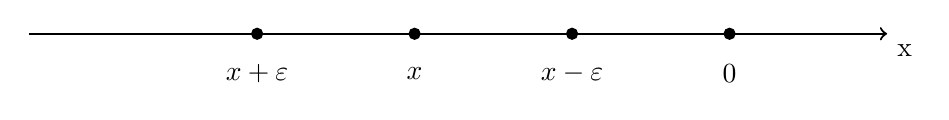
\begin{tikzpicture}
                \draw[thick,->] (-8.9,0) -- (2,0) node[anchor=north west] {x};
                \filldraw[black] (0,0) circle (2pt);
                \draw (0,-0.5) node{0};
                \filldraw[black] (-6,0) circle (2pt);
                \draw (-6,-0.5) node{\(x+\varepsilon\)};
                \filldraw[black] (-2,0) circle (2pt);
                \draw (-2,-0.5) node{\(x-\varepsilon\)};
                \filldraw[black] (-4,0) circle (2pt);
                \draw (-4,-0.5) node{\(x\)};
            \end{tikzpicture}
        \end{center}
    \end{proof} 
\end{theorem}

\newpage
\begin{theorem}
    If \(x_n\rightarrow x, y_n\rightarrow y\) are sequences in \(\R\) such that \(\forall n\in\N, x_n\le y_n\), 
    then \(x\le y\).

    \begin{proof}
        Consider \(z_n:=y_n-x_n\).
        Then \(z_n\ge 0\) and \(z_n\rightarrow y-x\) by the limit law.
        \[\Rightarrow y-x\ge 0\]
        \[y\ge x\]
    \end{proof}
\end{theorem}

\begin{theorem}
    If \(x_n\rightarrow x\) is a sequence in \(\R\), and let \(a,b\in\R\) such that 
    \(\forall n\in\N, a\le x_n\le b\), then \(a\le x\le b\).
    \begin{proof}
        Consider constant sequence \(a_n=a\) and \(b_n=b\). Then this is true by the last theorem.
    \end{proof}
\end{theorem}

\begin{theorem}[\textbf{Squeeze Theorem}]
    Suppose \(\seq{x}{n},\seq{y}{n},\seq{z}{n}\) are sequences of real numbers such that \(\forall n\in\N,x_n\le y_n\le z_n\).
    If \(\lim{\seq{x}{n}}=\lim{\seq{z}{n}}\), then \(\seq{y}{n}\) is convergent and 
    \[\lim{\seq{x}{n}}=\lim{\seq{y}{n}}=\lim{\seq{z}{n}}\]
    
    \begin{proof}
        Let \(\forall \varepsilon >0\).

        Write \(L=\lim{\seq{x}{n}}\). Then by definition of limit,
        
        \(\exists N_1\in\N \st \forall n\ge N\),
        \[\abs{x_n-L}<\varepsilon, \abs{z_n-L}<\varepsilon\]
        \begin{align*}
            \Rightarrow&& -\varepsilon<x_n-L&\le y_n-L\le z_n-L<\varepsilon\\
            \Rightarrow&& \abs{y_n-L}&<\varepsilon\\
        \end{align*}
        Thus \(\seq{y}{n}\) converges to \(L\) by definition of limit.\\
    \end{proof}
\end{theorem}

\begin{proposition}
    \(\ln{(n)}\) is divergent.
    \begin{proof}
        Since \(\ln(n)\) is unbounded, it is divergent.\\
    \end{proof}
\end{proposition}

\begin{exercise}
    \(\lim{\frac{3n^2+2n+1}{5n^2-4}}=\frac{3}{5}\)
    \[\lim{\frac{3n^2+2n+1}{5n^2-4}}=\lim{\frac{3+2\frac{1}{n}+\frac{1}{n^2}}{5-4\frac{1}{n^2}}}\]
    Notice that each term of \(\frac{1}{n}\) and \(\frac{1}{n^2}\) converges to 0. Thus by limit law, 
    \[\lim{\frac{3+2\frac{1}{n}+\frac{1}{n^2}}{5-4\frac{1}{n^2}}}=\frac{\lim{\{3+2\cdot 0+0\}}}{\lim\{5-4\cdot 0\}}=\frac{3}{5}\]
\end{exercise}

\begin{proposition}
    \((-1)^n\) is divergent.
    \begin{proof}[Proof:Exercise]
        
    \end{proof}
\end{proposition}

\begin{theorem}
    If \(x_n\rightarrow x\), then \(\abs{x_n}\rightarrow \abs{x}\)
    \begin{proof}[Sketch of the proof]:
        \[\abs{\abs{x_n}-\abs{x}}\le \abs{x_n-x}\]
        
    \end{proof}
\end{theorem}

\begin{theorem}
    Suppose \(\seq{x}{n}\) is a sequence of non-negative real numbers, satisfiying \(x_n\rightarrow x\).
    Then \(\sqrt{x_n}\rightarrow\sqrt{x}\).
    \begin{proof} Let \(\forall \varepsilon>0\)

        \highlight{Case1:} \(x=0\)

        \(\exists N\in\N \st \forall n\ge N\), \[\abs{x_n-0}<\varepsilon^2\]
        \[\Rightarrow \abs{\sqrt{x}-0}<\varepsilon\]

        \highlight{Case2:} \(x>0\)

        \(\exists N \st \forall n>N,\) \[\abs{x_n-x}<\sqrt{x}\cdot\varepsilon\]
        Notice that
        \begin{align*}
            \abs{\sqrt{x_n}-\sqrt{x}}&=\abs{\frac{x_n-x}{\sqrt{x_n}+\sqrt{x}}}\\
            &\le \frac{\abs{x_n-x}}{\sqrt{x}}<\varepsilon
        \end{align*}
    \end{proof}
\end{theorem}

\begin{theorem}
    Let \(\seq{x}{n}\) be a sequence of positive real numbers such that \(L=\lim(\frac{x_{n+1}}{n})\) exists. 
    If \(L<1\), then \(\seq{x}{n}\) converges to 0.

    \begin{proof}
        \(\exists N_1\in\N \st \forall n>N_1\)
        \[\abs{\abs{\frac{x_{n+1}}{x_n}}-\abs{L}}\le\abs{\frac{x_{n+1}}{x_n}-L}<\frac{1-L}{2}\]
        Thus \[\abs{\frac{x_{n+1}}{x_n}}<\frac{1+L}{2}\]

        Note that \(\frac{1+L}{2}<1\), write \(r=\frac{1+L}{2}\).
        Then \(\forall m\in\N\),
        \[x_{N_1+m}<x_{N_1+(m-1)}r<x_{N_1+(m-2)}r^2<\dots<x_{N_1}r^m\]
        Consider \(\seq{y}{m}=\seq{x}{N_1+m}\), \(\seq{z}{m}=(x_{N_1}r^m)\). Then 
        \[0\le y_m\le z_m\]
        Since \(z_m\rightarrow 0\)
        \[\seq{y}{m}\rightarrow 0 \text{ by squeeze theorem}\]
        Thus we conclude that \(\seq{x}{n}\rightarrow 0\) by m-th tail theorem.
    \end{proof}
\end{theorem}

\newpage
\subsection{Monotone sequence}

\begin{definition}
    Let \((x_n)\) be a sequence of real. We say \(\seq{x}{n}\) is ...
    \begin{itemize}
        \item \highlight{increasing} if \(\forall n\in\N, x_{n+1}\ge x_n\).
        \item \highlight{strickly increasing} if \(\forall n\in\N, x_{n+1} > x_n\).
        \item \highlight{decreasing} if \(\forall n\in\N, x_{n+1}\le x_n\).
        \item \highlight{strickly decreasing} if \(\forall n\in\N, x_{n+1}< x_n\).\\
    \end{itemize}
\end{definition}

\begin{theorem}[\textbf{Monotone Convergence Therorem}]
    A monotone sequence of real numbers is \highlight{convergent} iff it is bounded. 
Moreover, if \((x_n)\) is increaseing, then 
\[\lim(x_n) = \sup{\{x_n:n\in\N\}}\]
    If \((x_n)\) is decreasing, then 
    \[\lim(x_n) = \inf{\{x_n:n\in\N\}}\]
\end{theorem}

\begin{proof}\((\Rightarrow)\)

    A convergent sequence is always bounded.

    \((\Leftarrow)\) 
    
    Suppose \(\seq{x}{n}\) is a monotone and bounded sequence.

    \highlight{Case 1:} \(\seq{x}{n}\) is increasing.

    Write \(x = \sup{\{x_n:n\in\N\}}\).

    Let \(\varepsilon>0\). Since \(x = \sup{(x_n)}\):
    \[x-\varepsilon \text{ is NOT an upper boudn of } \seq{x}{n}\]
    Then 
    \[\exists N\in\N \st x_N > x-\varepsilon\]
    Since \(\seq{x}{n}\) is increasing,
    \[\forall n\ge N,\, x_n>x-\varepsilon\]

    On the other hand,\(x+\varepsilon\) is an supper bound since x is an upper bound. Thus,
    \[x_n<x+\varepsilon\]
    \[\Rightarrow \forall n\ge N, x-\varepsilon<x_n<x+\varepsilon\]
    \[\Rightarrow \abs{x_n - x}<\varepsilon\Rightarrow\seq{x}{n}\rightarrow x\]

    \highlight{Case 2:} \(\seq{x}{n}\) is decreasing.

    Write \(y = \inf{\seq{x}{n}}\). Let \(\varepsilon>0\)

    Since \(y = \inf{(x_n)}\),
    \[y+\varepsilon \text{is NOT and upper bound of }\seq{x}{n}\]
    Thus
    \[\exists N \in\N \st x_n<y+\varepsilon\]
    Since \(\seq{x}{n}\) is decreasing,
    \[\forall n>N, x_n<y+\varepsilon\]
    
    On the other hand, \(y-\varepsilon\) is a lower bound since \(y\) is a lower bound. Hence, 
    \[\forall n\in\N,  y-\varepsilon<x_n\]
    \[\forall n\ge N, y-\varepsilon<x_n<y+\varepsilon \Rightarrow\abs{x_n-y}<\varepsilon\]
    \[\Rightarrow \seq{x}{n}\rightarrow y\]

    \begin{remark}
        One can prove case 2 by following: 
        
        \(\seq{-x}{n}\) is increasing and converges to \(\sup{(-x_n)}\) by case 1.
        Also note that \[\seq{x}{n} = (-\seq{-x}{n})\rightarrow -\sup{\seq{-x}{n}}\]
        by limit law. So it is easy to prove that \[-\sup{(\seq{-x}{n})} = \inf{(x_n)}\]
    \end{remark}
\end{proof}

\begin{example}
    Consider the sequence \((x_n)\) is given by 
        \[\begin{cases}
            & x_0 = \frac{1}{2}\\
            & x_{n+1} = \frac{3}{2}x_n(1-x_n)\\
        \end{cases}\]

    \((x_n)\) is decreasing and  bounded.

    \highlight{Thoughts: } Assume \((x_n)\) converges, then by limit law,
    \[x = \frac{3}{2}x(1-x)\text{ where }x=\lim(x_n)\Rightarrow x = 0\text{ or }3\]
    then, by proof of contradiction, it is not convergent.
\end{example}

\begin{proof}
    \highlight{Claim}: \(\frac{1}{3}<x_{n+1}<x_n\le\frac{1}{2},\, \forall n \in \N \cup \left\{0\right\}\)\\\\
    \highlight{Proof of the claim by induction:} 

    When n = 0:
    \[x_0=\frac{1}{2},\, x_1 = \frac{3}{2}\cdot\frac{1}{2}(1-\frac{1}{2})=\frac{3}{8}\]
    \[\frac{1}{3}<\frac{3}{8}<\frac{1}{2}\le\frac{1}{2}\]

    Suppose this is true for n=k:
    \[\frac{1}{3}< x_{k+1}<x_k\le\frac{1}{2}\]

    Goal: \[\frac{1}{3}<x_{k+2}<x_{k+1}\le\frac{1}{2}\]
    \[x_{k+1} = \frac{3}{2}x_k(1-x_k)\]
    \[\frac{1}{3}<x_k\le\frac{1}{2}\,\Rightarrow\frac{2}{3}>1-x_k\ge\frac{1}{2}\]
    \[x_{k+1}<\frac{3}{2}\cdot\frac{1}{2}\cdot\frac{2}{3} = \frac{1}{2}\]
    Complete the square:
    \begin{align*}
        x_{k+1}-\frac{1}{3} & = \frac{3}{2}x_k(1-x_k)-\frac{1}{3}\\
        & = -\frac{3}{2}[(x_k-\frac{1}{2})^2-\frac{1}{36}]
    \end{align*}
    So
    \begin{align*}
        \frac{1}{3}<x_k\le\frac{1}{2}& \Rightarrow \abs{x_k-\frac{1}{2}}<\frac{1}{6}\\
        & \Rightarrow (x_k-\frac{1}{2})^2<\frac{1}{36}\\
        & \Rightarrow x_{k+1}-\frac{1}{3}>0\\
        & \Rightarrow \frac{1}{3}<x_{k+1}\le\frac{1}{2}
    \end{align*}
    With the similar process, we can derive that 
    \[\frac{1}{3}<x_{k+2}\le\frac{1}{2}\]
    \[x_{k+2} = \frac{3}{2}x_{k+1}(1-x_{k+1})<\frac{3}{2}x_{k+1}\cdot\frac{3}{2}=x_{k+1}\]
    Therefore, this claim is also true for n=k+1: \[\frac{1}{3}<x_{k+2}<x_{k+1}\le\frac{1}{2}\]
    We thereby prove the theorem by induction: 
    \[\frac{1}{3}<x_{n+1}<x_n\le\frac{1}{2}\]
\end{proof}

\highlight{Exercise: }
Textbook p.75: A sequence that converges to \(\sqrt{a}\) for \(a>0\).\newpage
\begin{definition}[\textbf{Euler's Number}]
    \[e = \lim(1+(\frac{1}{n})^n)\]
    \textbf{Goal: } \((x_n)\) is convergent where \(x_n=(1+\frac{1}{n})^n\)
    
    \begin{align*}
        x_n & = (1+\frac{1}{n})^n=1+nC1\cdot\frac{1}{n}+nC2\cdot\frac{1}{n^2}+\dots+nCn\frac{1}{n^n}\\
        & = 1+\frac{n}{1}\cdot\frac{1}{n}+\frac{n(n-1)}{2}\cdot\frac{1}{n^2}+\dots+\frac{n(n-1)\cdot3\cdot2\cdot1}{n!}\cdot\frac{1}{n^2}\\   
        & = 1 + 1+\frac{1}{2}(1-\frac{1}{n})+\frac{1}{6}(1-n)(1-\frac{2}{n})+\dots+\frac{1}{n!}(1-\frac{1}{n})(1-\frac{2}{n})\dots\frac{2}{n}\cdot\frac{1}{n}
    \end{align*}
    Write \(x_{n+1}\) in a similar way, we observe that \[x_n < x_{n+1}\]
    \highlight{Facts} \(2^{m-1}\le m!\) for \(m \in \N\Rightarrow \frac{1}{m!}\le\frac{1}{2^{m-1}}\)
    \[x_n<1+1+\frac{1}{2}+\frac{1}{4}+\dots+\frac{1}{2^{n-1}} = 1+\frac{1(1-(\frac{1}{2})^n)}{1-\frac{1}{2}}<3\]
    \(\Rightarrow(x_n) \)\text{ is increasing and bounded}
\end{definition}

\newpage

\subsection{Subsequence and the Bolzano-Weierstrass Theorem}
\begin{example}
    \begin{align*}
        (x_n) &= ((-1)^n)\\
        x_{2n} &= (-1)^{2n}\\
        x_{2n+1} &= (-1)^{2n-1}
    \end{align*}
    So \(a_n = x_{2n}\) is a sequence, while \(b_n = x_{2n+1}\) is a subsequence of \(x_n\).
\end{example}

\begin{definition}[\textbf{Subsequences}]
    Let \((x_n)\) be a real sequence and consider a strickly increasing seqence of natural numbers 
    \(n_1<n_2<n_3<\dots\)
    The sequence \[(x_{n_k}\,:\,k\in\N)\]
    is called a \highlight{subsequence} of \((x_n)\)\\
\end{definition}

\begin{example}
    Any tails of a sequence is a subsequence:
    \((x_n)\) n-th tail: \((x_{m+k})\), where \(n=m+k,k\in\N\), is a subsequence.\\
\end{example}

\begin{theorem}
    Suppose \((x_n)\) converges to \(x\). Then \(x_{x_k}\rightarrow x\) for any subsequence of \((x_n)\).
\end{theorem}
\begin{proof}
    Let \(\varepsilon > 0\), then 
    \[\exists N_\varepsilon >0 \text{ s.t. } \abs{x_n-x} < \varepsilon \text{ for }n>N_\varepsilon.\]
    Note that \[n_k \ge k,\,\forall k \in \N .\]
    \begin{exercise}
        By induction, \(n_1\ge 1, n_2 \ge n_1 \ge 1 \Rightarrow n_2 \ge 2\)
    \end{exercise}
    When \(k>N_\varepsilon,\, n_k>N_\varepsilon\), thus
    \[\abs{x_{n_k}-x}<\varepsilon\]
    Therefore\[(x_{n_k})\rightarrow x\]
\end{proof}

\begin{theorem}
    Let \((x_n)\) be a sequence of real numbers, and let \(x\in \R\). Then the following are equivalent:
    \begin{enumerate}
        \item \((x_n)\) does not converge to \(x\).
        \item \(\exists \varepsilon_0 >0, \text{ s.t. } \forall k \in \N, \exists n_k \in \N \text{ s.t. }\) 
        \[n_k\ge k\, \& \, \abs{x_{n_k}-x}>\varepsilon_0\]
        \item \(\exists \varepsilon_0 >0 \) and a subsequence \(\seq{x}{n_k}\) s.t. \[\abs{x_{n_k}-x}>\varepsilon_0,\, \forall k \in \N\]
    \end{enumerate}

    \begin{example}
        \[x_n = (-1)^n\Rightarrow\seq{x}{n}\text{ does not converge to 1}\]
    \end{example}

    \begin{proof}
        \begin{align*}
            3\rightarrow1 &\text{: by the contrapositive statement of definition} \\
            3\rightarrow2 &\text{: 3 is a stronger statement of 2} \\
            1\rightarrow2 &\text{: left as exercise}
        \end{align*}
    \end{proof}

\end{theorem}

\begin{theorem}
    If \(\seq{x}{n}\) satisfies either of the following property, then it is \highlight{divergent}:
    \begin{enumerate}
        \item There exists two subsequence \((x_{n_k})\) \& \((x_{m_k})\) whose limits are NOT equal.
        \item \((x_n)\) is unbounded.\\
    \end{enumerate}
\end{theorem}

\begin{example}
    \text{\\}
    \begin{enumerate}
        \item \((-1)^n\)
        \item \((n)\)
        \item \((x_n)\) such that \[x_{2k} = k\]\[x_{2k+1} = (-1)^k\]
    \end{enumerate}
\end{example}
\begin{proof}
    \textit{exercise}\\
\end{proof}

\begin{theorem}[\textbf{Bolzano-Weierstrass Theorem}]
    A bounded sequence of real numbers has a \highlight{convergent subsequence}.
    \begin{example}
        \[x_n = (-1)^n\]
    \end{example}
    \begin{proof}
        \begin{lemma}
            If \((x_n)\) is a sequence of real numbers, there exists a subsequence of \((x_n)\) which is monotone.
        \end{lemma}
        \highlight{proof of lemma:}\\
        Call the m-th term \(x_m\) a \textit{"peek"} if \(x_m\) is at least as large as any term after it in the sequence.
        
        \begin{center}
            \begin{tikzpicture}
                \draw[step=1cm,gray,very thin] (-0.9,-0.9) grid (3.9,3.9);
                \draw[thick,->] (-0.9,0) -- (4.9,0) node[anchor=north west] {x};
                \draw[thick,->] (0,-0.9) -- (0,4.9) node[anchor=south east] {y};
                \filldraw [black] (1,1) circle (2pt);
                \filldraw [black] (2,2) circle (2pt);
                \filldraw [black] (3,1.5) circle (2pt);
                \draw (3,1) node {"peek"};
            \end{tikzpicture}
        \end{center}

        \highlight{Case 1: }\((x_n)\) has infinitelyy many peaks

        List the peaks of \((x_n)\) in order of increasing index \[x_{n_1},x_{n_2},\dots\]
        \(\Rightarrow (x_{n_i})\) is a decreasing sequence.

        \highlight{Case 2: }\((x_n)\) has a finite number of peaks

        Let \(s_1\) be the first index after the last peak of \((x_n)\). Then for every \(n\ge s_1, \,\exists m\in\N\) such that \(x_m>x_n\).

        Choose \[s_2\ge s_1\text{ such that } x_{s_2}>x_{s_1},\, s_2\ge s_1\text{ such that } x_{s_2}>x_{s_1},\dots\]
        \[\Rightarrow (x_{s_i}) \text{ is an increasing sequence.}\]
        \begin{remark}
            Lemma + monotone convergent theorem implies Bolzano-Weierstrass theorem.
        \end{remark}

        \highlight{Second proof}

        Suppose \((x_n)\) is a bounded sequence.
        \[\Rightarrow \exists I_1=[a_1,b_1] \text{ such that }(x_n)\in I_1\]
        
        Consider \[I_2' = [a_1,\frac{a_1+b_1}{2}], \, I_2'' = [\frac{a_1+b_1}{2}, b_1]\]
        
        Let \(I_2 = [a_2,b_2]\) be one of \(I_2',I_2''\) such that \(I_2\) contains infinitely many terms of \((x_n)\).
        
        For \(n\in\N\), define \(I_n = [a_n,b_n]\) in a similar way.

        For \(i\in\N\), choose a term \(x_{n_i}\) such that \(x_{n_i}\in I_i\) and \(n_i>n_{i-1}\)

        Then \begin{align*}
            & i = 1,\, & n_i = 1\\
            & i = 2,\, & \text{choose }n_2\in\N \text{ such that } n_2>n_1 \,\& \,x_{n_2}\in I_2\\
            & \vdotswithin{=}\notag & \vdotswithin{=}\notag
        \end{align*}

        \begin{itemize}
            \item \(\forall i \in\N,\,a_i\le x_{n_i}\le b_i\)
            \item \((a_i) \text{ increases, bounded above by }b_1\Rightarrow (a_i)\rightarrow\sup{(a_i)}\)
            \item \((b_i) \text{ decreases, bounded below by }a_1\Rightarrow (b_i)\rightarrow \inf{(b_i)}\)
            \item \(\inf{\abs{a_i-b_i}} = \inf{\frac{b_1-a_1}{2^n}} = n \Rightarrow \sup{(a_i)} = \inf{(b_i)}\)
        \end{itemize}

        Thus \((x_{n_i})\) is convergent by squeeze theorem.\\
    \end{proof}
\end{theorem}

\begin{theorem}
    Let \((x_n)\) be a bounded sequence, and \(x\in\R\) has the property that every convergent subsequence of \((x_n)\) converges to \(x\). 
    Then \(x_n \text{ converges to } x\)
    \begin{proof}
        Let \(\forall\varepsilon>0\)

        By Bolzano-Weierstrass theorem, \(\exists\) a convergent subsequence \((x_{n_i})\) such that
        \[\exists N_\varepsilon\in\N \text{ s.t. for } i>N_\varepsilon, \abs{x_{n_i}-x}<\varepsilon\]
        
        Assume \((x_n)\) does not converge to \(x\). Then by previous theorem of subsequence,
        \[\exists \varepsilon_0 >0 \text{ and a subsequence }(x_{n_k}) \text{ s.t. }\abs{x_{n_k}-x}>\varepsilon_0, \forall k\in\N\]
        
        Since \((x_n)\) is bounded, \((x_{n_k})\) is also bounded. Thus there exists a convergent subsequence of \((x_{n_k})\) as \((x_{n_{k_i}})\).

        Note that \((x_{n_{k_i}})\) is a convergent subsequence of \((x_n)\), thus 
        \[(x_{n_{k_i}})\rightarrow x\text{ which is contradiction to previous assumption }\]
    \end{proof}
\end{theorem}

\begin{definition}
    Let \((x_n)\) be a sequence of real numbers. A point is called a \highlight{subsequential limit} of \((x_n)\) if it is the limit of a subsequence of \((x_n)\).
    \[S = \{\alpha \in\R:x\text{ is a subsequential limit}\}\text{ NOTE: may be infinite set}\]
\end{definition}

\begin{definition}
    Let \((x_n)\) be a sequence of real numbers.
    \begin{itemize}
        \item The \highlight{limit superior} of \((x_n)\) is the infimum of the set of \(v\in\R\) s.t. \(v< x_n\) for at most a finite number of \(n\in\N\). We write it as
        \[\limsup(x_n)\text{ or }\limsup x_n\text{ or }\overline{\lim}x_n\]
        \item The \highlight{limit inferior} of \((x_n)\) is the supremum of the set of \(v\in\R\) s.t. \(w >x_m\) for at most a finite number of \(n\in\N\). We write it as
        \[\liminf(x_n)\text{ or }\liminf x_n\text{ or }\overline{\lim}x_n\]
    \end{itemize}
\end{definition}

\highlight{Intuition} 

\begin{itemize}
    \item Suppose \(v<x_n\) for at most finitely many \(n\in\N\), then \\
\end{itemize}


\begin{theorem}
    Let \((x_n)\) be a bounded sequence, and \(x\in\R\) has the property that every convergent subsequence of \((x_n)\) converges to \(x\). 
    Then \(x_n \text{ converges to } x\)
    \begin{proof}
        Let \(\forall\varepsilon>0\)

        By Bolzano-Weierstrass theorem, \(\exists\) a convergent subsequence \((x_{n_i})\) such that
        \[\exists N_\varepsilon\in\N \text{ s.t. for } i>N_\varepsilon, \abs{x_{n_i}-x}<\varepsilon\]
        
        Assume \((x_n)\) does not converge to \(x\). Then by previous theorem of subsequence,
        \[\exists \varepsilon_0 >0 \text{ and a subsequence }(x_{n_k}) \text{ s.t. }\abs{x_{n_k}-x}>\varepsilon_0, \forall k\in\N\]
        
        Since \((x_n)\) is bounded, \((x_{n_k})\) is also bounded. Thus there exists a convergent subsequence of \((x_{n_k})\) as \((x_{n_{k_i}})\).

        Note that \((x_{n_{k_i}})\) is a convergent subsequence of \((x_n)\), thus 
        \[(x_{n_{k_i}})\rightarrow x\text{ which is contradiction to previous assumption}\]
    \end{proof}
\end{theorem}
\begin{definition}
    Let \((x_n)\) be a sequence of real numbers. A point is called a \highlight{subsequential limit} of \((x_n)\) if it is the limit of a subsequence of \((x_n)\).
    \[S = \{\alpha \in\R:x\text{ is a subsequential limit}\}\text{ (NOTE: may be infinite set)}\]
    \begin{example}
        Consider \(\seq{x}{n}=\{(-1)^n|n\in\N\}\). Then 
        \[S \supseteq \{1,-1\}\]
    \end{example}

\end{definition}

\begin{definition}[\(\limsup\) and \(\liminf\)]
    Let \((x_n)\) be a sequence of real numbers.
    \begin{itemize}
        \item The \highlight{limit superior} of \((x_n)\) is the infimum of the set of \(v\in\R\) s.t. \(v< x_n\) for at most a finite number of \(n\in\N\). We write it as
        \[\limsup(x_n) = \limsup x_n = \overline{\lim}x_n = \inf{\{v\in\R|v<x_n \text{ for at most a finite number of n}\}}\]
        \begin{example}
            Consider \(\seq{x}{n}=\frac{1}{n}\)
            \begin{center}
                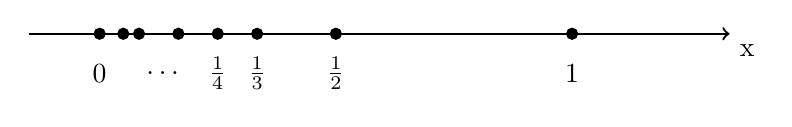
\begin{tikzpicture}
                    \draw[thick,->] (-0.9,0) -- (8,0) node[anchor=north west] {x};
                    \filldraw[black] (0,0) circle (2pt);
                    \draw (0,-0.5) node{0};
                    
                    \filldraw[black] (6,0) circle (2pt);
                    \draw (6,-0.5) node{1};

                    \filldraw[black] (3,0) circle (2pt);
                    \draw (3,-0.5) node{\(\frac{1}{2}\)};

                    \filldraw[black] (2,0) circle (2pt);
                    \draw (2,-0.5) node{\(\frac{1}{3}\)};

                    \filldraw[black] (1.5,0) circle (2pt);
                    \draw (1.5,-0.5) node{\(\frac{1}{4}\)};

                    \filldraw[black] (1,0) circle (2pt);

                    \filldraw[black] (0.5,0) circle (2pt);

                    \filldraw[black] (0.3,0) circle (2pt);
                    \draw (0.8,-0.5) node{\(\dots\)};

                \end{tikzpicture}
            \end{center}

            Let\[X=\{v\in\R|v<x_n \text{ for at most a finite number of n}\}\]
            \begin{itemize}
                \item \(-1\notin X\) because there are infinitely many \(x_n\) such that \(v<x_n\).
                \item \(\frac{1}{2}\in X\) because there are finitely many \(x_n\) such that \(v<x_n\).
                \item \(2\in X\) because there is no \(x_n\) such that \(v<x_n\), which is smaller than finite and thereby satisfies the definition.
            \end{itemize}

            We thus conclude that \[(0,\infty)\subset X\text{ and } \limsup{x_n} = \inf{X}\]
        \end{example}

        \begin{example}
            Consider \(\seq{x}{n} = (-1)^n\):
            \begin{center}
                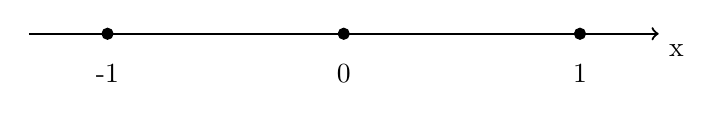
\begin{tikzpicture}
                    \draw[thick,->] (-4,0) -- (4,0) node[anchor=north west] {x};
                    \filldraw[black] (0,0) circle (2pt);
                    \draw (0,-0.5) node{0};
                    
                    \filldraw[black] (3,0) circle (2pt);
                    \draw (3,-0.5) node{1};

                    \filldraw[black] (-3,0) circle (2pt);
                    \draw (-3,-0.5) node{-1};

                \end{tikzpicture}
            \end{center}
            \begin{itemize}
                \item \(1\in X\) because there is no \(x_n\) such that \(v<x_n\).
                \item \(2\in X\) because there is no \(x_n\) such that \(v<x_n\).
                \item \(0,-1\notin X\) because there are infinitely many \(x_n\) such that \(v<x_n\).
            \end{itemize}
            We thus conclude that \[[1,\infty)\subset X\text{ (in fact they are equal)}\]
        \end{example}
        \item The \highlight{limit inferior} of \((x_n)\) is the supremum of the set of \(w\in\R\) s.t. \(w >x_m\) for at most a finite number of \(n\in\N\). We write it as
        \[\liminf(x_n)\text{ or }\liminf x_n\text{ or }\overline{\lim}x_n = \sup{\{w\in\R|w>x_n\text{ for at most a finite number of n}\}}\]
    \end{itemize}
\end{definition}
\newpage
\highlight{Intuition} 

\begin{itemize}
    \item Suppose \(v<x_n\) for at most finitely many \(n\in\N\), then for all large n, \(v\ge x_n\). \\\(\Rightarrow\) No subsequential limit of \(\seq{x}{n}\) can possibly exceed v.
    \item Similar observation for \(\underline{\lim{}}x_n\)\\
\end{itemize}


\begin{theorem}
    Let \((x_n)\) be a bounded sequence of real numbers, and let \(x^*\in\R\). Then TFAE:
    \begin{enumerate}
        \item \(x^* = \limsup(x_n)\)
        \item If \(\varepsilon>0\), there are at most a finite number of \(n\in\N\) s.t.
        \(x^*+\varepsilon <x_n\), but infinitely many n for which \(x^* - \varepsilon<x_n\)
        \item If \(u_m=\sup{\{x_n|n\ge m\}}\)(sup of (m-1)-th tail), then \(x*=\inf{\{u_m|m\in\N\}} = \lim{u_m}\)
        \item If \(S\) is the set of subsequential limits of \(x_n\), then \(x^*=\sup S\).\\
    \end{enumerate}

    \begin{remark}
        .
        \begin{itemize}
            \item \(u_m\) is decreasing.
            \item There is a similar such list of equivalent properties for \(\liminf\).\\
        \end{itemize}
    \end{remark}

    \begin{corollary}
        A bounded sequence \((x_n)\) is convergent iff \(\overline{\lim}x_n = \lim x_n\)
        \begin{proof}
            A direct result of the theorem:\[\overline{\lim}x_n=\sup{S} \text{ and } \underline{\lim}x_n=\inf{S}\]
        \end{proof}
    \end{corollary}

    \begin{proof}[Proof of thm. (a) \(\Rightarrow\) (b)]
        Let \(\varepsilon >0\). Then
        \[x^*+\varepsilon>x^* = X =\inf{\{v\in\R | v<x_n \text{ for at most a finite number of n.}\}}\]
        \[\Rightarrow \exists v\in\R \text{ s.t. } x^*\le v < x^*+\varepsilon\]
        and there are only finitely mant n with \(v<x_n\).
        
        For any \(n\) for which \(x^*+\varepsilon < x_n\), \(v<x_n\). Thus there are only finitely many such n.

        If \(x^*-\varepsilon \notin X\), then there are infinityly many \(n\) such that \(x^* - \varepsilon<x_n\)
    \end{proof}
    \newpage

    \begin{proof}[Proof of thm. (b) \(\Rightarrow\) (c)]
        Fix \(\varepsilon>0\).

        By (b), there are only finitely many n with \(x^*+\varepsilon<x\).

        Take \(N\in\N\) large enough such that
        \begin{align*}
            &&x^*+\varepsilon&\ge x_n&\forall n\ge N\\
            &\Rightarrow&x^*+\varepsilon &\ge u_N\\
            &\Rightarrow&x^*+\varepsilon &\ge \lim{u_n}\\
            &\Rightarrow&x^* &\ge \lim{u_m} &\forall n\ge N
        \end{align*}

        On the other hand, there are infinitely many n with \(x^*-\varepsilon<x_n\le u_n\).

        \(\text{Thus, there exists a subsequence of }u_n\text{, say }u_{n_k}\text{, satisfies}\)
        \begin{align*}
            &&x^*-\varepsilon&\le u_{n_k}\\
            &\Rightarrow &x^*-\varepsilon &\le \lim{u_{n_k}}=\lim{\seq{u}{n}}\\
            &\Rightarrow &x*&\le \lim{\seq{u}{n}}
        \end{align*}
    \end{proof}

    \begin{proof}[Proof of thm. (c) \(\Rightarrow\) (d)]
        \highlight{Goal}:
        \[x*=\lim{\seq{u}{m}}, u_m=\sup{x_n|n\ge m}\]
        \[\Rightarrow x^*=\sup{S} \text{ where S is the set of subsequential limits.}\]

        Let \(\seq{x}{n_k}\) be a convergent subsequence of \(\seq{x}{n}\). Notice that \(\lim{\seq{x}{n_k}}\in S\).
        \begin{align*}
            &&n&\ge k\\
            &\Rightarrow&x_{n_k} \le \sup{\{x_n|n\ge k\}}=u_k\\
            &\Rightarrow&\lim{\seq{x}{n_k}} \le \lim{\seq{u}{k}}=x^*\\
            &\Rightarrow&x^* \text{ is an upper bound of S.}.
        \end{align*}

        For 1, \(\exists n_1\in\N \st\)
        \[u_1-1\le x_{n_1}\le u_1\]
        For \(\frac{1}{2}\), \(\exists n_2\in\N \st\)
        \[u_2-\frac{1}{2}\le x_{n_2}\le u_2\]
        \[\dots\]
        For \(\frac{1}{k}\), \(\exists n_k\in\N \st\)
        \[u_k-\frac{1}{k}\le x_{n_k}\le u_k\]
        When \(k\rightarrow \infty\),
        \[x^*-0\le \lim{\seq{x}{n_k}}\le x^*\]
        By squeeze theorem,
        \[\lim{\seq{x}{n_k}}=x^*\]
    \end{proof}

    \begin{proof}[Proof of thm. (d) \(\Rightarrow\) (a)]
        \highlight{Goal:}
        \[x^*=\sup{S}\]
        \[\Rightarrow x^*=\limsup{x_n}=\inf{\{v\in\R | v<x_n \text{for at most finite many of n}\}}\]

        Fix \(\varepsilon>0\)

        There is no subsequence of \(x_n\) which has a limit exceeding \(x^*+\varepsilon\).
        \begin{align*}
            &\Rightarrow \text{ There is only finitely many n with }x_n>x^*+\varepsilon.\\
            &\Rightarrow &x^*+\varepsilon&\in X\\
            &\Rightarrow &\inf{X} &\le x^*+\varepsilon\\
            &\Rightarrow &\limsup{x_n}&\le x^*+\varepsilon\\
            &\Rightarrow &\limsup{x_n}&\le x^*
        \end{align*}

        Next, consider \(x^*-\varepsilon\)

        Then, there exists a subsequential limit of \(x_n\) which is greater or equal to \(x^*-\frac{1}{2}\varepsilon\).
        
        There exists a convergent subsequence of \(\seq{x}{n}\), say \(\seq{x}{n_k}\), such that 
        \begin{align*}
            &&\lim{\seq{x}{n_k}}\ge x^*-\frac{1}{2}\varepsilon\\
            &\Rightarrow&\text{ There are infinitely many n with } x^*&>x^*-\varepsilon.&\\
            &\Rightarrow&\forall a\in X, x^*-\varepsilon &\le a\\
            &\Rightarrow&x^*-\varepsilon &\le \inf{X}\\
            &\Rightarrow&\limsup{x_n}&\ge x^*-\varepsilon\\
            &\Rightarrow&\limsup{x_n}&\ge x^*
        \end{align*}
        
        In conclusion, \[\limsup{x_n}=x^*\]

    \end{proof}
\end{theorem}
\newpage

\subsection{Cauchy Criterion}
\begin{definition}[\textbf{Cauchy Sequence}]
    A sequence \(\seq{x}{n}\) is \highlight{Cauchy sequence} if 
    
    \(\forall \varepsilon>0, \exists H\in\N \st \forall n,m\in\N, n>0,m>0\),
    \[\abs{x_n-x_m}<\varepsilon\]

    \begin{example}(\(\frac{1}{n}\)) is a Cauchy sequence.
        \begin{proof}
            Observe that \(\forall n,m\in\N, n\ge m\),
            \[\abs{\frac{1}{n}-\frac{1}{m}}=\abs{\frac{m-n}{mn}}=\frac{n-m}{mn}\le\frac{n}{mn}<\frac{1}{m}\]
            Choose \(H=\lceil \frac{1}{\varepsilon} \rceil+1\), Then

            \(\forall n,m\ge H\),
            \[\abs{\frac{1}{n}-\frac{1}{m}}\le \frac{1}{m}<\varepsilon\]
        \end{proof}
    \end{example}

    \begin{example}\((-1)^n\) is not a Cauchy sequence.
        \begin{proof}
            Choose \(\varepsilon_0=\frac{1}{2}, \forall H\in\N,\) choose \(n,m\ge H \st n\) is even, \(m\) is odd. Then 
            \[\abs{(-1)^n-(-1)^m}=\abs{1-(-1)}=2>\frac{1}{2}\]
            Thus \((-1)^n\) does not satisfies the definition of Cauchy sequence.\\
        \end{proof}
    \end{example}
\end{definition}

\begin{theorem}
    If \(\seq{x}{n}\) is convergent, then it is Cauchy sequence.
    \begin{proof}
        Let \(\lim{\seq{x}{n}}=x\).

        \highlight{Goal:} \[\abs{x_n-x}<\varepsilon\Rightarrow\abs{x_n-x_m}<\varepsilon\]
        \(\forall n,m\ge N_\varepsilon,\)
        \begin{align*}
            \abs{x_n-x_m} &= \abs{(x_n-x)+(x-x_m)}\\
            &\le \abs{x_n-x}+\abs{x-x_m} \text{ by triangle inequality}\\
            &<\frac{1}{2}\varepsilon+\frac{1}{2}\varepsilon=\varepsilon
        \end{align*}
    \end{proof}
\end{theorem}
\newpage

\begin{lemma}
    If \(\seq{x}{n}\) is Cauchy, the it is bounded.
    \begin{proof}
        Choose \(\varepsilon=1,\exists H\ge 0 \st \forall n,m\ge H\),
        \[\abs{x_n-x_m}<1\]
        Since the choice of \(m\) satisfies \(m\ge H\), we may choose \(m=H\st\)
        \[\abs{x_n-x_H}<1\]
        It follows that 
        \[\abs{x_n}-\abs{x_H}\le\abs{x_n-x_H}<1\]
        \[\abs{x_n}<\abs{x_H}+1,\forall n\ge H\]
        Let 
        \[M:=\max{\{\abs{x_1},\abs{x_2},\abs{x_3},\dots,,\abs{x_{H-1}},\abs{x_H}+1\}}\]
        Thus \(\forall n\in\N, \abs{x_n}\le M\)
    \end{proof}
\end{lemma}

\begin{theorem}[\textbf{Cauchy Convergence Theorem}]
    A sequence of real numbers is \highlight{convergent} if and only if it is \highlight{Cauchy} sequence.
    \begin{proof}[(\(\Rightarrow\))]
        Done in the previous theorem.
    \end{proof}
    \begin{proof}[(\(\Leftarrow\))]
        Suppose \(\seq{x}{n}\) is Cauchy. By lemma, it is bounded.

        By Bolzano-Weierstrass theorem, there exists a convergent subsequence \(\seq{x}{n_k}\). 
        
        Let \(\lim\seq{x}{n_k}=x\).

        \highlight{Goal:} \(\forall \varepsilon>0, \exists N\in\N \st \forall n\ge N\)
        \[\abs{x_n-x}<\varepsilon\]
        We will use the trick of \highlight{insert subsequence:}

        By definition of convergence, \(\forall \varepsilon>0, \exists N_\varepsilon\in\N \st \forall k\ge N_\varepsilon\)
        \[\abs{x_{n_k}-x}<\frac{1}{2}\varepsilon\]
        By definition of Cauchy sequence, \(\forall \varepsilon>0, \exists H\in\N,H\ge 0 \st \forall n,m\ge H\)
        \[\abs{x_n-x_m}<\frac{1}{2}\varepsilon\]
        
        Thus \(\forall k\ge \max\{H,N_\varepsilon\}\),
        \begin{align*}
            \abs{x_k-x} &= \abs{(x_k-x_{n_k})+(x_{n_k}-x)}\\
            &\le \abs{x_k-x_{n_K}}+\abs{x_{n_k}-x}\text{ since }n_k\ge k\ge \max\{H, N_\varepsilon\}\\
            &<\frac{1}{2}\varepsilon+\frac{1}{2}\varepsilon=\varepsilon
        \end{align*}
    \end{proof}
\end{theorem}
\newpage
\begin{example}
    Let \(\seq{h}{n}\) be the sequence of harmonic series such that 
    \[h_n=\sum_{i=1}^{n}\frac{1}{i}\text{ , and } \lim\seq{h}{n}=\sum_{n=1}^{\infty}\frac{1}{n}\]
    \highlight{Claim:} \(\seq{h}{n}\) is divergent 

    \highlight{Goal:} show that it is NOT Cauchy.
    \begin{proof}
        \(\forall m,n\in\N, \text{ WLOG suppose }m\ge n, h_m>h_n\), we have 
        \begin{align*}
            \abs{h_m-h_n}&=\frac{1}{n+1}+\frac{1}{n+2}+\dots+\frac{1}{m-1}+\frac{1}{m}\\
            &\ge \frac{m-n}{n}
        \end{align*}
        since there are (m-n)'s terms on the right side of the equation. 

        So we choose \(\varepsilon_0=\frac{1}{2},\forall H\ge 0, \text{ choose }n=H,m=2H\), then
        \[\abs{h_m-h_n}\ge \frac{m-n}{m}=\frac{1}{2}\]
        Thus, \(\seq{h}{n}\) is NOT Cauchy.
    \end{proof}
\end{example}
\newpage

\subsection{Property of Divergent Sequence}
\begin{example}[divergent sequence]:
    \begin{itemize}
        \item \((n)\rightarrow\infty\)
        \item \((-n)\rightarrow -\infty\)
        \item \((-1)^n\cdot n\) is divergent and unbounded.
        \item \((-1)^n\) is divergent and bounded.\\
    \end{itemize}
\end{example}

\begin{definition}[\textbf{Properly Divergent}]
    Let \(\seq{x}{n}\) be a sequence of real numbers. We say that 
    \begin{enumerate}
        \item \(\seq{x}{n}\) \highlight{tends to} \(\infty\), or \(\lim\seq{x}{n}=\infty\) if \(\forall a\in\R,\exists N\in\N \st \forall n\ge N\),
        \[x_n>a\]
        \item Similarly, \(\seq{x}{n}\) \highlight{tends to} \(-\infty\), or \(\lim\seq{x}{n}=-\infty\) if \(\forall a\in\R,\exists N\in\N \st \forall n\ge N\),
        \[x_n<a\]
    \end{enumerate}

    In either case, we say that \(\seq{x}{n}\) is \highlight{properly divergent}.\\
\end{definition}
\begin{example}
    Let \(C>0\). \((C^n)\) is properly divergent. We write \(\lim (C^n)=\infty\).
    \begin{proof}
        Notice that \[C^n=[1+(C-1)]^n\ge 1+n(C-1)\text{ by Bernoulli's inequality}\]
        \highlight{Goal:} \(\forall a\in\R, \exists N\in\N \st \forall n\ge N,\)
        \[1+n(C-1)>a_n\Leftrightarrow n>\frac{a_n-1}{C-1}\]

        Then we choose \(N=\lceil \frac{a-1}{c-1}\rceil+1\). Thus \(\forall n\ge N,C^n>a\).\\
    \end{proof}
\end{example}

\begin{theorem}
    A monotone sequence is \highlight{divergent} if and only if it is \highlight{bounded}.
    \begin{proof}
        \textit{Exercise.}
    \end{proof}
\end{theorem}

\begin{theorem}[\textbf{Comparison Test}]
    Let \(\seq{x}{n}\) and \(\seq{y}{n}\) be two sequences. Suppose \(\forall n\in\N,x_n\ge y_n\). Then,
    \begin{enumerate}
        \item If \(\seq{x}{n}\rightarrow\infty\), then \(\seq{y}{n}\rightarrow\infty\).
        \item If \(\seq{y }{n }\rightarrow - \infty\), then \(\seq{x }{n }\rightarrow -\infty\).
    \end{enumerate}
    \begin{proof}
        \textit{Exercise.}
    \end{proof}
\end{theorem}
\newpage
    
\begin{theorem}[\textbf{Limit Comparison Test}]
    Let \(\seq{x}{n}\) and \(\seq{y}{n}\) be two sequences of positive real numbers. Suppose \(\exists L\in\R,L>0\st\)
    \[\exists \lim(\frac{x_n }{y_n })=L\]
    then \(\lim(x_n)=\infty\) if and only if \(\lim(y_n)=\infty\)
\end{theorem}

\begin{proof}
    \highlight{Claim:} For N large enough, 
    \[\frac{1}{2}L\cdot y_n<x_n<2L\cdot y_n\]
    \highlight{Goal:} Claim+Comparison Theorem=Proof.

    By definition of limit, \(\forall \varepsilon>0, \exists N\in\N \st \forall n>N\),
    \[L-\varepsilon<\frac{x_n }{y_n }<L+\varepsilon\]
    Choose \(\varepsilon=\frac{1}{2}L\), we have 
    \[\frac{1}{2}L\cdot y_n<x_n<\frac{3}{2}L<2L\cdot y_n\]
    since \(L>0\) and these are positive sequences.

    Thus by Comparison Theorem, 
    \[\lim\seq{\frac{1}{2}L\cdot y}{n}=\infty\Rightarrow \lim\seq{x }{n }=\infty\]
\end{proof}
\newpage

\subsection{Introduction to Infinite Series}

\begin{definition}[\textbf{Infinite Series}] 
    If \(\seq{x }{n }\) is a sequence of real numbers, then the \highlight{infinite series} generated by \(\seq{x }{n }\) is the sequence \(\seq{s }{k }\) defined by 
    \[s_k=\sum_{i=1}^{k }x_i \]
    Terms \(s_k \) are called \highlight{partial sums}.\\
    \begin{notation}
        \(\sum x_i \) to mean this series or its limit at infinity \(\lim \seq{x }{ k }\).\\
    \end{notation}
\end{definition}

\begin{theorem}[\textbf{Cauchy Criterion for Series}] 
    The series \(\sum x_i \) \highlight{converges} if and only if \(\forall \varepsilon >0, \exists M\in\N \st \forall n,m\in\N, n>m\ge M\),
    \[\abs{x_{m+1}+x_{m+2}+\dots+x_{n-1}+x_{n}}<\varepsilon\]
    Or we write it as 
    \[\abs{s_k-s_m}<\varepsilon\]
    \begin{proof}[\textit{Proof: Exercise.}]
    \end{proof}
\end{theorem}

\begin{theorem}[Montone Convergence for Series]
    Let \(\seq{x }{n }\) be a sequence of non-negative real numbers. Then the series \(\sum x_n \) \highlight{converges} if and only if \(\seq{s }{k }\) is bounded.
    \begin{proof}
        \textit{Exercise.\\}
    \end{proof}
    \begin{example}
        \(\sum \frac{1}{n^2}\) is convergent.

        \begin{proof}
            \highlight{Goal:} find convergent subsequence \(\seq{s }{k_j }\).

            Consider subsequence \(\seq{s }{k_j }\) where \(k_j=2^j-1 \).

            Observe that:
            \begin{align*}
                s_{k_1}&=1\\
                s_{k_2}&=1+\frac{1}{2^2}+\frac{1}{3^2}\\&<s_{k_1}+2\cdot \frac{1}{2^2}=1+\frac{1}{2}\\
                s_{k_3}&=1+(\frac{1}{2^2}+\frac{1}{3^2})+(\frac{1}{4^2}+\frac{1}{5^2}+\dots+\frac{1}{9^2})\\&<s_{k_1}+2\cdot \frac{1}{2^2}=1+\frac{1}{2}
            \end{align*}
            By induction(details are left as exercise), one can show that 
            \[s_{k_j}<\sum_{n=0}^{j-1}\frac{1}{2^n }<\sum_{n=0}^{\infty}\frac{1}{2^n}=2\text{ (by limit of geometric series.)}\]
            Thus \(\seq{s }{k_j }\) is bounded.

            By theorem proved in homework, an increasing sequence with bounded(and thus convergent) subsequence implies that the sequence is convergent.
        \end{proof}
    \end{example}
\end{theorem}


\newpage

\section{Limits}

\subsection{Limits of Functions}
Let \(f:A\rightarrow B\) be a function where \(A,B\subseteq \R\). Let \(a\in A,L\in B\).

\highlight{Goal:} Define \[\lim_{x\rightarrow a}f(x)=?\]
\highlight{Intuition:} Define \textbf{\emph{closeness}} on real line.\\
\begin{definition}[\textbf{Cluster Point}]
    Let \(A\subseteq \R\). A point \(c\in\R\) is a \highlight{cluster point} of \(A\) if \\
    
    \(\forall \delta>0,\exists x\in A, x\neq c\) such that 
    \[\abs{x-c}<\delta\]
    Or 
    \[V_\delta (c)\cap (A \ \{c\})\neq \phi\]
    \linebreak
    
    \begin{center}
        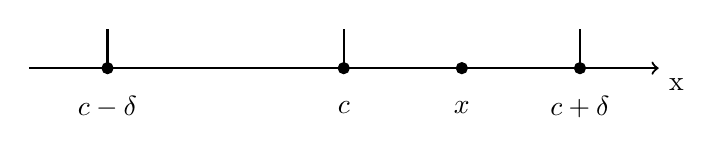
\begin{tikzpicture}
            \draw[thick,->] (-4,0) -- (4,0) node[anchor=north west] {x};
            \draw[thick] (-3,0) -- (-3,0.5);
            \draw[thick] (3,0) -- (3,0.5);
            \draw[thick] (0,0) -- (0,0.5);

            \filldraw[black] (0,0) circle (2pt);
            \draw (0,-0.5) node{\(c\)};

            \filldraw[black] (1.5,0) circle (2pt);
            \draw (1.5,-0.5) node{\(x\)};
            
            \filldraw[black] (3,0) circle (2pt);
            \draw (3,-0.5) node{\(c+\delta\)};

            \filldraw[black] (-3,0) circle (2pt);
            \draw (-3,-0.5) node{\(c-\delta\)};

        \end{tikzpicture}
    \end{center}
\end{definition}

\begin{theorem}
    \(c\in\R\) is a cluster point if and only if 

    there exists a sequence \(\seq{a}{n}\in A\) such that 
    \[\lim\seq{a }{n }=c \text{ and }\forall n\in\N, a_n\neq c\]

    \begin{proof}[Sketch of Proof](\(\Rightarrow\))
        \begin{align*}
            &\delta=1, \exists a_1 \in A \textbackslash \{c \} \st \abs{a_1-c}<1\\
            &\delta=\frac{1}{2}, \exists a_2\in A \textbackslash \{c \} \st \abs{a_2-c }<\frac{1}{2}\\
            &\dots\text{ observe that: }\\
            &\forall \delta>0, \exists a_n\in A \textbackslash \{c\} \st \abs{a_n-c}<\frac{1}{n }<\delta\\
            &\Rightarrow \lim\seq{a }{n}=c\text{ by squeeze theorem.}
        \end{align*}

        (\(\Leftarrow\))

        \(\forall\delta>0,\exists N_\varepsilon>0\st\)
        \[\abs{a_{N_\varepsilon}-c}<\delta\]
        Note that \(a_{N_\varepsilon}\in A\textbackslash\{c\}\) where \(c\) is a cluster point of \(A\).
    \end{proof}
    \newpage

    \begin{example}
        Let \(X\) be the set of cluster points of A. 

        \begin{itemize}
            \item \(A=(1,2)\cup (3,4)\Rightarrow X=[1,2]\cup [3,4]\). 
            \textit{Proof: Exercise.}
            \item \(A=\{0\}\cup (1,2)\Rightarrow X=\phi\).
            \begin{proof}[Sketch of (2)]:
                \begin{enumerate}
                    \item Let \(x\in[1,2]\). Prove that \(x\in X\). Thus \([1,2]\in X\).
                    \item Prove that \(0\notin X\).
                    \item Prove that \(x\in X\) if \(x\notin \{0\}\cup [1,2]\).
                \end{enumerate}
            \end{proof}
        \end{itemize}
    \end{example}

    \begin{remark}
        \(A\) may not be a subset of the set of cluster points of \(A\).
        \begin{example}:
            \begin{itemize}
                \item \(A=\Z\Rightarrow X=\phi\).
                \item \(A=\{\frac{1}{n }|\,n\in\N \}\Rightarrow X=\{0\}\) \textit{Proof: Exercise.}\\
            \end{itemize}
        \end{example}
    \end{remark}
\end{theorem}

\begin{definition}[\textbf{Delta-Epsilon Definition of Limit}]
    Let \(A\subseteq\R\), \(c\) is a cluste point of \(A\), \(f:A\rightarrow\R\). A real number L is the \highlight{limit of f at c} if 

    \(\forall \varepsilon>0, \exists\delta>0 \st \forall x\in A,\)
    \[0<\abs{x-c }<\delta \rightarrow \abs{f(x)-L}<\varepsilon\]
\end{definition}

\begin{theorem}[\textbf{Uniqueness of Limit}]
    If \(f:A\rightarrow \R\) and \(c \) is a cluster of points of \(A \), then \(f \) has at most 1 limit at \(c \).
    \begin{proof}
        We will prove this by contradiction.

        Let \(L_1\) and \(L_2\) be limits of \(f \) at \(c \). Assume \(L_1\neq L_2 \). Choose \(\varepsilon=\frac{\abs{L_1-L_2}}{2}>0\). Then,
        \[\exists \delta_1\st 0<\abs{x-c}<\delta_1\Rightarrow\abs{f(x)-L_1}<\frac{\varepsilon}{2}\]
        \[\exists \delta_2\st 0<\abs{x-c}<\delta_2\Rightarrow\abs{f(x)-L_2}<\frac{\varepsilon}{2}\]
        Consider \(\delta:=\min\{\delta_1,\delta_2\}\). 

        Since \(c\) is a cluster point, \(\exists x_0\in A\st\) 
        \[0<\abs{x_0-c}<\delta\]
        Since \[\abs{f(x_0)-L_1}<\frac{\varepsilon}{2},\abs{f(x_0)-L_2}<\frac{\varepsilon}{2}\]
        We have 
        \begin{align*}
            \abs{L_1-L_2}&\le \abs{L_1-f(x_0)}+\abs{f(x_0)-L_2}\\
            &<\frac{\varepsilon}{2}+\frac{\varepsilon}{2}=\varepsilon\\
            &=\frac{\abs{L_1-L_2}}{2}
        \end{align*}
        which is a contradiction.\\
    \end{proof}
\end{theorem}

\begin{notation}
    \[L=\lim_{x\rightarrow c}f(x)\text{ or } L=\lim_{x\rightarrow c}f\]
    And we say that \textit{f(x) approaches to L as x approaches to c}.\\
\end{notation}

\begin{remark}[\textbf{Divergence of function}]
    If the limit of \(f(x)\) at \(c\) does not exists, we say that \(f\) \highlight{diverges} at \(c\).\\
\end{remark}

\begin{theorem}
    Let \(f:A\rightarrow \R\) and \(c \) be a cluster point of \(f \). The following are equivalent:
    \begin{enumerate}
        \item \(\lim_{x\rightarrow c }f(x)=L\)
        \item \(\forall\, V_\varepsilon(L)\,\varepsilon\text{-neighborhood of L, }\exists\, V_\delta(c)\,\delta\text{-neighborhood of }c\st\)
        \[x\in V_\delta(c)\cap (A\backslash\{c\})\Rightarrow f(x)\in V_\varepsilon(c)\]
    \end{enumerate}
    \centerfig{LimitFunction.png}
\end{theorem}

\begin{example}
    \(\lim_{x\rightarrow c}f(x)=a\).
    \begin{proof}
        \(\forall \varepsilon>0, \exists\delta=1\st\)
        \[x\in \neighbor{\delta}{c}\cap(\R\backslash\{c\})\Rightarrow f(x)=a\in\neighbor{\varepsilon}{L}\]
    \end{proof}
\end{example}

\begin{example}
    \(\lim_{x\rightarrow c}f(x)=c\).
    \begin{proof}
        \(\forall \varepsilon>0,\exists \delta=\varepsilon\st\)
        \begin{align*}
            &x\in\neighbor{\delta }{c }\cap (A\backslash\{c \})\\
            \Rightarrow& f(x)=x\in\neighbor{\delta }{c }\cap(A\backslash\{c \})\\
            \Rightarrow&f(x)\in\neighbor{\varepsilon }{c }\cap(A\backslash\{c \})\subseteq \neighbor{\varepsilon }{c }
        \end{align*}
        
    \end{proof}
\end{example}

\newpage
\begin{example}
    \[\limx{c }{x^2}=c^2\]
    \begin{proof}
        \highlight{Goal}: \(\forall \varepsilon>0\), find a \(\delta(c,\varepsilon)>0\) \st
        \[\text{if }0<\abs{x-c}<\delta\text{, then }\abs{x^2-c^2}<\varepsilon\]
        which is equivalent to show
        \[\abs{x+c}\abs{x-c}<\varepsilon\]

        Since the choice of \(\delta\) is dependent on \(\varepsilon\) and \(c\) only, \(\abs{x-c}\) can be easily confined with some constant. 
        Let's assume that
        \[\abs{x-c}<1\]
        Now, the only task left is to find a way to confine \(\abs{x+c}\) with a constant by manipulating \(\abs{x-c}<1\). 

        Here we will apply a common trick that estimates addition \(\abs{x+c}\) with subtraction \(\abs{x-c}\):
        \[\abs{x}-\abs{c} \le \abs{x-c} < 1 \text{ by triangle inequality.}\]
        Rearranging the inequality, we have:
        \[\abs{x}<\abs{c}+1\]
        Adding the second \(\abs{c}\) to both side of inequality, then, we apply triangle inequality again:
        \[\abs{x+c}\le\abs{x}+\abs{c}<2\abs{c}+1\]
        \[\abs{x+c}<2\abs{c}+1\]
        Notice that this is equivalent to show
        \[\abs{x+c}\abs{x-c}<(2\abs{c}+\delta)\abs{x-c}<\varepsilon\]
        Rearrange the constant factor \[\abs{x-c}<\frac{\varepsilon}{2\abs{c}+1}\]
        Thus, our choice of \(\delta\) must satisfies two conditions at the same time:

        \begin{equation*}
            \begin{cases}
                \abs{x-c}<1 \\
                \abs{x-c}<\frac{\varepsilon}{2\abs{c}+1}
            \end{cases}
        \end{equation*}
        We achieve this by simply choosing
        \[\delta=\min\left\{\frac{\varepsilon}{2\abs{c}+1},1\right\}\]
    \end{proof}
\end{example}

\begin{remark}[\highlight{The Toolbox of Proofs}]
    The readers should develop their "toolbox" of proof techniques. 
    That is, the \highlight{estimation against a constant} + manipulation of \highlight{triangle inequality} + choice of \(\delta\) that satisfies \highlight{multiple conditions}.
\end{remark}

\newpage
\begin{example}[Harder]
    \[\limx{c}{\frac{1}{x}}=\frac{1}{c}\]
    \begin{proof}        
        Observe that
        \[\abs{\frac{1}{x }-\frac{1}{c}}=\frac{\abs{x-c}}{\abs{cx}}\]
        Here, we cannot choose \(\abs{x-c}\) smaller than some constant(why? try it on your own). Instead,
        we choose \[\abs{x-c}<\frac{\abs{c }}{2 }\]
        By triangle inequality,
        \[\frac{\abs{c }}{2 }<\abs{x}<\frac{3\abs{c }}{2 }\]
        Multiply \(\abs{c}\) to each term of the inequality,
        \[\frac{c^2}{2 }<\abs{cx}<\frac{3c^2}{2 }\]
        Thus
        \[\frac{1 }{\abs{cx }}<\frac{2 }{c^2 }\]
        It follows that 
        \[\frac{\abs{x-c }}{\abs{cx }}<\frac{2}{c^2}\abs{x-c }\]
        In order to make the left term of the inequality less than \(\varepsilon\), 
        it suffices to confine 
        \[\frac{2}{c^2}\abs{x-c}<\varepsilon\]
        \[\abs{x-c}<\frac{c^2}{2}\varepsilon\]

        Thus, our choice of \(\delta\) must satisfies two conditions at the same time:
        \begin{equation*}
            \begin{cases}
                \abs{x-c}<\frac{\abs{c }}{2 } \\
                \abs{x-c}<\frac{c^2}{2}\varepsilon
            \end{cases}
        \end{equation*}
        We achieve this by simply choosing
        \[\delta=\min\left\{\frac{\abs{c }}{2 },\frac{c^2}{2}\varepsilon\right\}\]

    \end{proof}
\end{example}

\begin{remark}[\highlight{Factoring }\(\abs{x-c}\)]
    Since we have the premice of \(\abs{x-c }<\delta\) for free, it would be much easier for us to 
    confine \(\abs{f(x)-L}\) if we factor \(\abs{x-c}\) from the difference.
\end{remark}

\newpage

\begin{example}[Much Harder]
    \[\forall n\in\N, \limx{c }{x^n }=c^n\]
    \begin{proof}
        By difference of \(n\)-th powers factorization
        \[\abs{x^n-c^n }=\abs{x-c}\abs{\sum_{i=0}^{n-1 }x^i c^{n-1-i}}\le \abs{x-c }\cdot\sum_{i=0}^{n-1 }\abs{x}^i \abs{c}^{n-1-i}\]
        If \[\abs{x-c }<1\]
        then by triangle inequality,
        \[\abs{x }<\abs{c }+1\]
        It follows that
        \[\abs{x^n-c^n}<\abs{x-c}\cdot\sum_{i=0}^{n-1 }(\abs{c}+1)^i \abs{c^{n-1-i}}\]
        Similar to the previous example, it suffices to confine 
        \[\abs{x-c}\cdot\sum_{i=0}^{n-1 }(\abs{c}+1)^i \abs{c^{n-1-i}}<\varepsilon\] 
        \[\abs{x-c}<\frac{\varepsilon}{\sum_{i=0}^{n-1 }(\abs{c}+1)^i \abs{c^{n-1-i}}}\]
        Thus, choose 
        \[\delta =\min\{1, \frac{\varepsilon}{\sum_{i=0}^{n-1 }(\abs{c}+1)^i \abs{c^{n-1-i}}}\}\]
    \end{proof}
\end{example}

\begin{remark}[\highlight{Estimate \(x\) against \(c\)}]
    This is another trick by triangle inequality:
    
    If \(\exists k\in\R,k>0\st\abs{x-c }<k\), then \(\abs{x}<\abs{c}+k\)\\
\end{remark}

\begin{remark}[\highlight{difference of \(n\)-th powers factorization}]
    \[(x^n-c^n)=(x-c)(x^{n-1}+cx^{n-2}+\dots+c^{n-2}x+c^{n-1})=(x-c)\sum_{i=0}^{n-1 }x^i c^{n-1-i}\]
\end{remark}

\newpage

\begin{example}[\highlight{Some Tedious Factorization}]
    \[\limx{2}{\frac{x^3+2x-1}{6x^2-5}}=\frac{11}{19}\]
    \begin{proof}
        \[\abs{\frac{x^3+2x-1}{6x^2-5}-\frac{11}{19}}=\abs{\frac{19x^3-66x^2+38x+36}{19(6x^2-5)}}\]
        By some tedious factorization,
        \[...=\abs{x-2}\frac{\abs{19x^3-28x-18}}{19\abs{6x^2-5}}\]
        We estimate \(\abs{x-2 }\) with constant 1
        \[\abs{x-2}<1\]
        \[1<x<3\text{ or }\abs{x }<3\]
        It follows that 
        \[1<x^2<9\]
        \[1<6x^2-5<49\]
        \[1>\frac{1}{6x^2-5}>\frac{1}{49}\]
        So
        \[\frac{1}{19\abs{6x^2-5}}<\frac{1}{19}\]
        Similarly,
        \[\abs{19x^3-66x^2+38x+36}\le19\abs{x}^2+28\abs{x}+18 <19\cdot3^2+28\cdot3+18=273\]
        Thus
        \[...\le \abs{x-2}\cdot\frac{273}{19}<\varepsilon\]
        \[\abs{x-2}<\frac{19}{273}\varepsilon\]
        We conclude that it suffices to choose 
        \[\delta=\min\left\{1, \frac{19}{273}\varepsilon\right\}\]

    \end{proof}
\end{example}
\newpage

\begin{theorem}[\highlight{Sequential Criterion of Limits}]
    Let \(f:A\rightarrow\R\) and let \(c \) be a cluster point of A. \(\limx{c }{f }=L\) if and only if 
    for all sequence \(\seq{x }{n }\in A\) that converge to \(c \) and \(\seq{x }{n }\neq c, \forall n \in \N\), 
    \((f(x_n))\) converges to \(L \).

    \begin{proof}[Proof. \((\Rightarrow)\)]
        By definition of convergent sequence, \(\forall \delta>0, \exists K\in\N \st \forall n\in\N, n\ge K,\) 
        \[\abs{x_n-c}<\delta\]
        By definition of limit, \(\forall \varepsilon>0, \exists \delta>0 \st \forall x\in A,\) 
        \[\abs{x-c}<\delta\Rightarrow\abs{f(x )-L}<\varepsilon\]
        Thus, choose \(\delta\) given \(\varepsilon\), and choose \(K\) given \(\delta\), we have:
        \[\abs{x_n-c}<\delta\Rightarrow\abs{f(x_n)-L}<\varepsilon\]
    \end{proof}

    \begin{proof}[\((\Leftarrow)\)]
        We will prove this by contrapositive.

        Assume that there exists \(\varepsilon_0>0\) and a \(\seq{x }{n }\in A \) converges to \(c \) with \(\seq{x }{n }\neq c\) 
        such that for all \(n\in\N\)
        \[0<\abs{x_n-c}<\frac{1}{n}\Rightarrow\abs{f(x_n)-L}\ge\varepsilon_0\]
        Thus the function does not have a limit at \(c\). We thereby conclude the converse of the statement.\\
    \end{proof}

\end{theorem}

\begin{theorem}[\highlight{Sequential Criterion of Divergence}]
    Let \(A\subseteq\R,f:A\rightarrow\R\), \(c \) be a cluster point of \(A\), 
    \(\seq{x }{n }\rightarrow c\st\seq{x }{n }\neq c\), and \(L\in\R\)\footnote{The following theorems are NOT equivalent!!}.
    \begin{enumerate}
        \item \(L\) is NOT the limit of \(f\) at \(c\) \(\iff\) \(f(x_n)\) does NOT converge to \(L\).
        \item \(f\) diverges \(\iff\) \(f(x_n)\) does NOT converge.
    \end{enumerate}

    \begin{proof}[Proof. Exercise.]
    \end{proof}
\end{theorem}

\begin{example}
    \[\limx{0}{\dfrac{1}{x }}\text{ does NOT exists in } \R\]
    \begin{proof}
        Let \(\seq{x }{n }=\frac{1 }{n }\rightarrow 0\). Then 
        \[f(x_n)=\dfrac{1}{\frac{1}{n}}=n\rightarrow\infty\]
    \end{proof}
\end{example}

\newpage
\begin{example}
    \[\limx{0}{\sin(\frac{1}{x })} \text{ DNE in } \R\]
    \centerfig{diverge-sin.jpg}
    \begin{proof}
        Let \(\seq{x }{n }=\dfrac{1 }{2n\pi}\rightarrow 0\) and \(\seq{y }{n }=\dfrac{1 }{\dfrac{1}{2}\pi + 2n\pi}\rightarrow 0\). Then 
        \[f(x_n)=\sin(2n\pi)=0\]
        \[f(y_n)=\sin(\dfrac{1}{2}\pi+2n\pi)=1\]
        Thus limit of \(f\) at \(0\) does NOT exists in \(\R\).\\
    \end{proof}
\end{example}

\begin{example}
    \begin{definition}[\highlight{Signum Function}] Let \(A\subseteq\R\) and \(sgn(x):A\rightarrow\R\st\)
        \[sgn(x)=\begin{cases}
            1 & \text{if }x>0\\
            0 & \text{if }x=0\\
            -1 & \text{if }x<0
        \end{cases}\]
    \end{definition}

    \[\limx{0}{sgn(x)}\text{ DNE in }\R\]
    \begin{proof}
        Let \(\seq{x }{n }=\dfrac{1 }{n}\rightarrow 0\) and \(\seq{y }{n }=\dfrac{1 }{-n}\rightarrow 0\). Then 
        \[f(x_n)=sgn(n)=1\]
        \[f(y_n)=sgn(-n)=-1\]
        Thus limit of \(f\) at \(0\) does NOT exists in \(\R\).\\
    \end{proof}

\end{example}
\newpage

\subsection{Limit Theorem}

\begin{definition}[\highlight{Bounded Neighborhood of c}]
    Let \(A\subseteq\R,f:A\rightarrow\R\), \(c \) be a cluster point of \(A\). 
    Then we say \(f\) is a \highlight{bounded Neighborhood of c} if 
    there exists \(\delta>0\text{ and }\exists M>0\st\forall x\in A\cap\neighbor{\delta}{c }\)
    \[\abs{f(x )}\le M\]
\end{definition}

\begin{theorem}[\highlight{Existence of Bounded Neighborhood at Limit}]
    If \(f\) has a limit at \(c\), then \(f\) is bounded on some neighborhood of \(c\).
    \begin{proof}
        By definition of limit, \(\forall \epsilon>0, \exists \delta>0 \st \forall x\in A\backslash\{c \}\)
        \[0<\abs{x-c}<\delta\Rightarrow\abs{f(x)-L}<\epsilon\]
        By triangle inequality,
        \[\abs{f(x)}-\abs{L}\le\abs{f(x)-L}<\epsilon\]
        \[\abs{f(x)}<\abs{L}+\epsilon\]
        If \(f(c)\) is not defined on \(A\), then let \(M=\abs{L}+\epsilon\). If \(f(c)\) is defined on \(A\), 
        then let \(M=\max\{f(c), \abs{L}+\varepsilon\}\). Since the choice of \(\varepsilon\) is arbitrary, 
        we will choose \(\epsilon=1\). Thus, 
        \[f(x)\le M\]
    \end{proof}
\end{theorem}

\begin{definition}
    Let \(A\subseteq\R;\ f,g:A\rightarrow\R\), \(c \) be a cluster point of \(A\). Then \(\forall x\in A\)
    \begin{itemize}
        \item \highlight{Sum} of function: \((f+g)(x)=f(x)+g(x)\).
        \item \highlight{Difference:} \((f-g)(x)=f(x)-g(x)\).
        \item \highlight{Multiple: } \((bf)(x)=b\cdot f(x)\) for some \(b\in \R\).
        \item \highlight{Product:} \((f\cdot g)(x)=f(x)\cdot g(x)\).
        \item \highlight{Quotient:} \((\dfrac{f}{g})(x)=\dfrac{f(x)}{g(x)}\) if \( g(x)\neq 0\).\\
    \end{itemize}
\end{definition}

\begin{theorem}[\highlight{Limit Theorem}]
    If \(\exists L,M\in R\st\limx{c }{f(x )}=L \) and \(\limx{c }{g(x )}=M\), then 
    \begin{itemize}
        \item \(\limx{c}{(f+g)(x)}=L+M\).
        \item \(\limx{c}{(f-g)(x)}=L-M\).
        \item \(\limx{c}{(bf)(x)}=b\cdot L\).
        \item \(\limx{c}{(f\cdot g)(x)}=L\cdot M\).
        \item \(\limx{c}{(\dfrac{f}{g})(x)}=\dfrac{L }{M}\) if \(\limx{c }{g(x )}\neq 0\).
    \end{itemize}

    \begin{proof}[Proof. Exercise.]
        
    \end{proof}
\end{theorem}

\begin{remark}
    Always check conditions befor applying: this is true only if both \(f\) and \(g\) has a limit at \(c\) !
\end{remark}

\newpage
\begin{example}
    \(\displaystyle\limx{4}{\frac{(x-4)(x+3)}{4(x-4)(x-5)}}=\limx{4}{\frac{x+3}{4(x-5)}}=-\frac{7}{4}\)\\
\end{example}

\begin{corollary}[\hypertarget{polynomial-functions}{\highlight{Polynomial Function}}]
    \[\limx{c }{p(x)}=\limx{c }{\sum_{i=0}^{n}a_i\cdot x^i}=\sum_{i=0}^{n}a_i\cdot\limx{c }{x^i}=\sum_{i=0}^{n}a_i\cdot x^i=p(c)\]
\end{corollary}

\begin{corollary}[\hypertarget{rational-functions}{\highlight{Rational Function}}]
    For polynomial functions \(\ds p(x),q(x)\st \\\limx{c}{p(x)}\rightarrow p(c), \limx{c}{q(x)}\rightarrow q(c)\neq 0\),
    \[\limx{c }{\frac{p(x )}{q(x )}}=\frac{p(c )}{q(c )}\]
\end{corollary}

\begin{theorem}
    Let \(A\subseteq\R;\ f,g:A\rightarrow\R\), \(c \) be a cluster point of \(A\). 
    
    If \(\exists a,b\in\R, \forall x\in A, x\neq c\) satisfiying 
    \[a\le f(x)\le b\text{ and }\limx{c}{f}=L\]
    then \[a\le\limx{c}{f}\le b\]
    \begin{proof}
        \(\ds \forall \seq{x }{n }\in A\backslash\{c\}, \seq{x }{n }\rightarrow c,\)
        \[a\le f(x_n)\le b\Rightarrow a\le L \le b\]
    \end{proof}
\end{theorem}

\begin{theorem}[\highlight{Squeeze Theorem}]
    Let \(A\subseteq\R;\ f,g,h:A\rightarrow\R\), \(c \) be a cluster point of \(A\). 

    If \(\ds\forall x\in A, x\neq c\), \[f(x)\le g(x) \le h(x)\text{ and }\limx{c}{f}=L=\limx{c}{h}\]
    then 
    \[\limx{c }{g}=L\]
    \begin{proof}[Proof. Exercise. Try sequeeze theorem of sequence.]
    \end{proof}
\end{theorem}

\begin{example}
    \(\ds\limx{0 }{x\sin(\frac{1 }{x})}=0\)
    \begin{proof}
        Notice that
        \[-1\le \sin(\frac{1}{x })\le 1\Rightarrow-x\le x\sin(\frac{1}{x })\le x\]
        Since 
        \[\limx{0}{(-x)}=0=\limx{0}{(x)}\]
        \[\limx{0}{x\sin(\frac{1}{x })}=0\]
    \end{proof}
\end{example}

\newpage
\begin{example}
    Let \(\ds b\in\R, b>0\). Then \(\ds\limx{0}{x^b}=0\).
    Notice that when \(x\in[0,1]\)
    \[x^{\left\lceil b \right\rceil}\le x^b<x^{\left\lfloor b \right\rfloor}\]
    The rest is left as exercise.
\end{example}

\begin{theorem}
    Let \(A\subseteq\R;\ f,g,h:A\rightarrow\R\), \(c \) be a cluster point of \(A\). 
    If \(\ds\limx{c }{f }>0\), then \(\ds \exists \delta>0\st\neighbor{\delta}{c}\st \forall x\in A\cap\neighbor{\delta}{c }\backslash\{c\}\),
    \[f(x)>0\]
    \begin{proof}[Proof. Excercise.]
        
    \end{proof}
\end{theorem}

\newpage
\section{Continuous Functions}
\subsection{Continuity}
\begin{definition}[\highlight{Counituous}]
    Let \(A\subseteq\R,\ f:A\rightarrow\R\), \(c \in A\). 

    We say \(f \) is \highlight{countinuous at c} if 

    \(\forall \varepsilon>0, \exists \delta>0 \st \forall x\in A\)
    \[\abs{x-c}<\delta\Rightarrow\abs{f(x)-f(c)}<\varepsilon\]

    We say \(f\) is \highlight{discontinuous at c} if \(f\) is NOT continuous at c.\\
\end{definition}

\begin{definition}[\highlight{Using Neighborhood}]
    Let \(A\subseteq\R,\ f:A\rightarrow\R\), \(c \in A\). Then \(f\) is continuous at \(c\) if and only if\\
    \(\forall \varepsilon>0 \text{ and its } \varepsilon \text{-neighborhood at }f(c),\ \neighbor{f(c)}{\varepsilon},\ \exists \delta>0 \text{ and its }\delta \text{-neighborhood at c },\ \neighbor{c}{\varepsilon},\ \st\)
    \[f(\neighbor{\delta}{c}\cap A)\subseteq \neighbor{\varepsilon }{f(c )}\]
    \centerfig[0.9]{def-conti-nbhd.jpg}
\end{definition}

\begin{remark}[\hypertarget{conti-criterion}{\highlight{Comparison with Limit Definition}}]\ 
    Continuity has 3 good properties that will be useful in the future study of Real Analysis:
    \begin{itemize}
        \item If c is a \highlight{cluster point} of \(A\), then \(f\) is \highlight{continuous} if and only if
        \begin{enumerate}
            \item \(f(x)\) is defined at c.
            
            \textbf{Counter-example:} Any function \(f:\Q\rightarrow\R\) is \textit{undefined} at \(\R\backslash\Q\) and thus \textit{discontinuous} at \(\R\backslash\Q\).

            \item \(\ds\limx{c }{f(x )}\) exists.\\
            \textbf{Counter-example:} \(\ds \frac{1}{x} \) is \textit{undefined} at 0 and thus \textit{discontinuous} at 0.

            \item \(\ds f(c)=\limx{c }{f(x )}\).\\
            \textbf{Counter-example:} \(\ds f(x)=\begin{cases}
                1, & \text{if }x\neq 0 \\
                0, & \text{if }x=0
            \end{cases}\) is discontinuous at 0 as \\ \(\ds f(c) = 0 \neq 1=\limx{c }{f(x )}\)
        \end{enumerate}
        \item If c is \highlight{NOT a cluster point} of A, then c is an \highlight{isolated point}, and
        
        \(\ds \exists\neighbor{\delta}{c }\cap A=\{c \}\). Notice that an \highlight{isolated point} is \highlight{automatically continuous} 
        as it \textit{satisfies} the definition of continuity at c. This is because
        \[\abs{x-c}=\abs{c-c}=0<\delta\Rightarrow\abs{f(x)-f(c)}=\abs{f(c)-f(c)}=0<\varepsilon\]
    \end{itemize}
\end{remark}

\begin{theorem}[\highlight{Sequential Criterion for Continuity}]\ 

    Let \(A\subseteq\R,\ f:A\rightarrow\R\), \(c \in A\). Then \(f\) is continuous at \(c\) if and only if 
    
    \(\forall \seq{x }{n }\subseteq A\ \st\seq{x }{n }\rightarrow c,\ f(\seq{x }{n })\rightarrow f(c)\).
    \begin{proof}[Proof. \((\Rightarrow)\)]
        Continuity of \(f\) at c implies limit of \(f\) at c exists\footnote{proof by definition}. Thus we simply apply sequential criterion of limit.

        \((\Leftarrow)\). This is exactly the statement of sequential criterion for limit at c. Thus, 
        \[\exists\limx{c }{f(x)}=f(c)\]
        Notice that \(c\in A\) implies that f is defined on \(c\). Thus, we conclude that \(f\) is continuous on c by previous \hyperlink{conti-criterion}{remark in p.43}
    \end{proof}
\end{theorem}

\begin{corollary}[\highlight{Sequential Criterion for Discontinuity}]\ 

    Let \(A\subseteq\R,\ f:A\rightarrow\R\), \(c \in A\). Then \(f\) is discontinuous at \(c\) if and only if 
    
    \(\exists \seq{x }{n }\subseteq A\ \st\seq{x }{n }\rightarrow c,\ f(\seq{x }{n })\not\rightarrow f(c)\).
    \begin{proof}[Proof. Similar. Left to reader as exercise.]
        \ \\
    \end{proof}
\end{corollary}

\begin{example} We begin with polynomial and rational functions:
    \begin{itemize}
        \item Constant function \(f(x)=b\) is continuous in \(\R\).
        \item Linear function \(f(x)=ax+b\) is continuous in \(\R\).
        \item Quadratic function\(f(x)=x^2\) is continuous in \(\R\).
        \item \(f(x)=\dfrac{1}{x^2}\) is continuous in \(\R\).
        \item \hyperlink{polynomial-functions}{Polynomial functions} are continuous in \(\R\)(try to prove it!).
        \item \hyperlink{rational-functions}{Rational functions} are continuous in \(\R\)(try to prove it!).
        \item \(f(x)=\dfrac{1}{x}\) is NOT continuous at 0.
        \item \(f(x)=sgn(x)\) is NOT continuous at 0.\\
    \end{itemize}
\end{example}

\newpage

\begin{example}[\highlight{Dirichlet’s ‘‘discontinuous function’’}]\ 

    Let \(A=\R\) and define Dirichlet’s ‘‘discontinuous function’’ by 
    \[f(x)=\begin{cases*}
        1 & if \(x\in\Q\) (rational)\\
        0 & if \(x\in\R\backslash\Q\) (irrational)
    \end{cases*}\]
    \highlight{Claim:} this function is discontinuous on \(\R\).
    \begin{proof}
        Let \(c\in A\).
        \begin{itemize}
            \item If \(c\in\Q\), then \(\ds\exists \seq{x }{n }\in \R\backslash\Q\ \st\forall n\in\N,\)
            \[c<\seq{x }{n }<c+\frac{1 }{n }\]
            By squeeze theorem,
            \[\lim{c}\le\lim{\seq{x }{n }}\le\lim{(c+\frac{1}{n})}\]
            \[\seq{x}{n }\rightarrow c,\ (c+\frac{1}{n})\rightarrow c\]
            \[\lim{f(x_n)}=1\neq0=\lim{f(c+\dfrac{1}{n })}\]
            Thus, by Sequential Criterion of Discontinuity, \(f\) is discontinuous for all \(c\in\Q\).
            \item If \(c\in\R\backslash\Q\), then we adopt similar strategy. The rest of proofs is left as exercise.
        \end{itemize}
    \end{proof}
\end{example}

\begin{example}[\highlight{Thomae’s function}] *Notice that this example is harder. We skip it on class.

    Let \(f:\R^+\rightarrow \R\) defined by 
    \[f(x)=\begin{cases*}
        0 & if \(x\in \R\backslash\Q\) (irrational)\\
        \frac{1}{q} & if \(x=\frac{p}{q}\in\Q\) (rational)
    \end{cases*}\]
    \highlight{Claim:} \(f\) is discontinuous on \(\Q\) and continuous on \(\R^+\backslash\Q\).
    \centerfig{thomae's-function}
    \begin{proof}\ 
        \begin{itemize}
            \item If \(c\) is rational, then \(\exists\seq{x }{n }\in\R^+\backslash\Q+\st \seq{x }{n }\rightarrow c\). Then we have 
            \[\lim f(x_n)\rightarrow 0\neq \dfrac{1}{q}=f(c)\]
            Since funtion value does not equal to limit value at c, \(f\) is discontinuous at \(c\in\Q\)
            \item If \(c\) is irrational,
            \highlight{Goal:} show that \(\forall \varepsilon>0, \exists \delta>0\st \forall x\in R^+,\)
            \[\abs{x-c}<\delta\Rightarrow\abs{f(x)-f(c)}=\abs{f(x)}<\varepsilon\]
            \begin{itemize}
                \item If \(x\in \R^+\backslash\Q\), then \(\abs{f(x)}=0<\varepsilon\) for some arbitrary choice of \(\delta\).
                \item If \(x\in \Q\), then by Archimedean Property, we could find a \(\frac{1}{n_0}>\varepsilon\). 
                
                Notice that there are only finite number of \(n\in\N\) such that \(n<n_0\). Thus, there are only 
                finite number of \(\dfrac{p}{q}\in(c-1,c+1)\) with denominator \(q<n_0\). Hence we could choose \(\delta\) so small that 
                the \(\neighbor{\delta }{c }\) contains no rational numbers with denominator less than \(n_0\). It follows that 
                \[\abs{x-b}<\delta \Rightarrow \abs{f(x)-f(c)}=\abs{f(x)}\le \dfrac{1}{n_0}<\epsilon\]
                Thus, \(f\) is continuous at \(c\in\R\backslash\Q\)
                
            \end{itemize}
        \end{itemize}
    \end{proof}
\end{example}

\newpage
\subsection{Combinations of Continuous Functions}
\begin{theorem}
    Let \(A\subseteq\R,\ f,g:A\rightarrow\R\), \(c \in A\), \(b\in R\). Suppose \(f,\ g\) are \highlight{continuous} on \(c\), then the following combination of functions are \highlight{continuous}:
    \begin{itemize}
        \item \highlight{Addition:} \(f+g\)
        \item \highlight{Subtraction:} \(f-g\)
        \item \highlight{Product:} \(f\cdot g\)
        \item \highlight{Multiplication:} \(b\cdot f\)
        \item \highlight{Quotient:} \(\dfrac{f }{g}\) if \(g(x)\neq 0\)
        \item \highlight{Absolute:} \(\abs{f}(x)\)
        \item \highlight{Square Root:} \(\sqrt{f}(x)\)
    \end{itemize}
    \begin{proof}\ 
        \begin{itemize}
            \item If \(c\) is not a cluster point of \(A\), then the theorem is automatically correct.
            \item If \(c\) is a cluster point of \(A\), then we only need to show that the function value 
            at \(c\) is equal to the limit of function at \(c\). Detailed proof are left as exercise.
        \end{itemize}
    \end{proof}
\end{theorem}
\begin{example}
    \begin{itemize}\ 
        \item Polynomial functions are continuous on \(\R\). 
        \item Rational functions are continuous on \(\R\).\\
    \end{itemize}
\end{example}

\begin{example}\ 
    \begin{itemize}
        \item \(\sin(x)\) is continuous on \(\R\).
        \begin{proof}
            Notice that \(\forall x, y, z\in \R\), we have 3 inequalitis:
            \[\abs{\sin(z)\le \abs{z},\ \abs{\cos(z)}\le 1},\ \sin(x)-\sin(y)=2\sin[\dfrac{1}{2}(x-y)]\cdot \cos[\dfrac{1}{2}(x+y)]\]
            Hence if \(c\in\R\), we have 
            \[\abs{\sin(x)-\sin(c)}\le 2\cdot \frac{1}{2}\abs{x-c}\cdot 1=\abs{x-c}\]
            Thus \(\sin(x)\) is continuous on \(\R\).
        \end{proof}
        \item \(\cos(x)\) is continuous on \(\R\)
        \begin{proof}[Proof. Exercise]
            Similar techniques as above.
        \end{proof}
        \item \(\tan(x),\ \cot,\ \sec,\ \csc\) are all continuous on \textit{where they are defined}.
        \begin{proof}
            Combinations of continuous functions on their domain are continuous.\\
        \end{proof}
    \end{itemize}
\end{example}

\begin{theorem}
    Let \(A,B\subseteq\R,\ f:A\rightarrow\R,\ g:B\rightarrow\R,\ c \in A\, \st f(A)\subseteq B\). Suppose \(f\) is continuous at \(c\in A\), 
    \(g\) is \highlight{continuous} on \(b=f(c)\in B\), then the composition \(g \circ f\) is \highlight{continuous} at \(c\). 
    
    \begin{proof}
        Since \(f\) is continuous at \(c\), \(\forall \varepsilon>0,\ \exists \delta>0\ \st\forall x\in A\), 
        \[\abs{x-c}<\delta\Rightarrow\abs{f(x)-f(c)}<\varepsilon\]
        Since \(g\) is continuous at \(b=f(c),\ f(A)\subseteq B\), \(\forall \zeta>0,\ \exists \varepsilon>0\ \st\forall f(x)\in B\), 
        \[\abs{f(x)-b}<\varepsilon\Rightarrow\abs{g(f(x))-g(b)}<\zeta\]
        Thus,
        \[\abs{x-c}<\delta\Rightarrow\abs{g(f(x))-g(b)}=\abs{g\circ f(x)-g\circ f(c)}<\zeta\]
    \end{proof}
    \centerfig[0.6]{composition-function}
\end{theorem}

\begin{example}
    \(\sqrt{x^2+1}\) is continuous on \(\R\).
    \begin{proof}[Proof. Exercise]        
    \end{proof}
\end{example}

\newpage

\subsection{Continuous Function on Bounded Intervals}
Continuous function on \highlight{closed bounded interval} has many good properties.\\

\begin{definition}[\highlight{Bounded Function}]
    A function \(f:A\rightarrow\R\) is said to be \highlight{bounded on A} if \(\exists M>0\st\forall x\in A\)
    \[\abs{f(x)}\le M\] 
    A function is \highlight{unbounded} if \(\forall M>0,\ \exists x_M\in A\st\)
    \[\abs{f(x)}>M\]
\end{definition}

\begin{example}
    \(\ds f(x)=\frac{1}{x }\) is unbounded on \(A=(0,\infty)\).
    \begin{proof}
        By Archimedean Property, \(\forall M>0,\exists x_M=\frac{1}{M+1}\in A\st\)
        \[\abs{f(\frac{1}{M+1})}=\abs{\frac{1}{\frac{1}{M+1}}}=\abs{M+1}>M\]
        We thereby conclude that \(\dfrac{1}{x}\) is unbounded on \(A\).
    \end{proof}
\end{example}

\begin{theorem}[\highlight{Boundness Theorem}]
    Let \(a,b\in\R,\ a<b,\ I=[a,b]\) a \highlight{closed bounded interval}. If \(f:I\rightarrow\R\) is countinuous on \(I\), 
    then \(f\) is bounded on \(I\).
    \begin{proof}
        Assume \(f\) is not bounded on \(I\). Then, by definition, \(\forall n\in\N,\ \exists x_n\in I\st\)
        \[\abs{f(x_n)}>n\]
        Since \(I\) is bounded, the sequence \(\seq{x }{n }\in I\) is bounded. Therefore, 
        by the Bolzano-Weierstrass Theorem, there exists a convergent subsequence \(\seq{x}{n_k}\rightarrow x\) for some number \(x\in I\). 
        Since \(f\) is continuous on \(I\), \[f(x_{n_k})\rightarrow f(x)\]
        We thereby conclude that \(f(x_{n_k})\) is a bounded sequence, which is a contradiction to unboundedness of \(f(x_{n_k})\)
        \[\forall k\in\N, n_k\in\N,\ \abs{f(x_{n_k})}>n_k\ge k\]
    \end{proof}

    \begin{remark}
        We will give 3 counter-examples to show that all of three conditions are necessary for Boundedness Theorem to be true.
        \begin{itemize}
            \item Interval must be \highlight{closed}\\
            \textbf{Counter-example:} \(f(x)=\dfrac{1}{x }\) on \((0,1]\) is countinous but unbounded.
            \item Interval must be \highlight{bounded}\\
            \textbf{Counter-example:} \(g(x)=x\) is continuous but unbounded on \([0,\infty)\).
            \item The function must be \highlight{continous}\\
            \textbf{Counter-example:} Define \(h:[0,1]\rightarrow\R,\ h(x)=\begin{cases*}
                \frac{1}{x} & if \(x\in(0,1]\)\\
                1 & if \(x=0\)
            \end{cases*}\) is discontinuous and unbounded.
            
        \end{itemize}
    \end{remark}
\end{theorem}
\newpage
\begin{definition}[\highlight{Maximum and Minimum}]
    Let \(A\in\R,\ f:A\rightarrow\R\). 
    
    We say that \(f\) has an \highlight{absolute maximum} on \(A\) if 
    \(\exists x^*\in A\st\forall x\in A\)\[f(x^*)\ge f(x)\]
    We say that \(f\) has an \highlight{absolute minimum} on \(A\) if 
    \(\exists x_*\in A\st\forall x\in A\)\[f(x_*)\le f(x)\]
\end{definition}

\begin{remark}
    Continuous function on a \highlight{bounded set A} does not necessarily have an maximum or minimum 
    on \(A\). For example:
    \begin{itemize}
        \item \(f(x)=\dfrac{1}{x}\) has NO absolute maximum or absolute minimum on \(A=(0,\infty)\)
        \item \(g(x)=x^2\) has only absolute minimum \(x_*=0\) on \(\R\).\\
    \end{itemize}
\end{remark}

\begin{theorem}[\highlight{Maximum-Minimum Theorem}]
    Let \(I=[a,b]\in\R\) be a \highlight{closed bounded} \highlight{interval}, \(f:I\rightarrow\R\) be \highlight{countinuous} on \(I\). Then \(f\) has an absolute maximum 
    and absolute minimum on \(I\). 
    \begin{proof}
        By previous theorem, \(f\) is bounded on \(I\). Thus, 
        \[\exists s^*=\sup f(I), \beta=\inf f(I)\]
        We will first proof that \(f\) has an absolute maximum. It suffices to 
        show that \[\exists x^*\in I\st f(x^*)=\sup f(I)\]
        Since \(s^*=\sup f(I)\), then \(\forall n\in\N, s^*-\dfrac{1}{n}\) is not an upper bound of the set \(f(I)\).\\
        Consequently, \(\exists x_n\in I\st\forall n\in\N\)
        \[s^*-\frac{1}{n }<f(x^*)\le s^*\]
        Since \(I\) is bounded, \(\seq{x }{n }\) is bounded, by the Bolzano-Weierstrass Theorem, 
        there exists a subsequence \(\seq{x }{n_k }\in I\st\seq{x }{n_k }\rightarrow x^*\).\\
        Since \(f\) is continuous on \(I\),
        \[\lim(f(x_{n_k}))=f(x*)\]
        By squeeze theorem,
        \[\lim (s^*-\frac{1}{n_k })\le\footnote{The reader should find out why the strict inequality become weak inequality when limit applies.} \lim f(x_{n_k})\le \lim s^*\]
        \[s^*\le f(x^*)\le s^*\]
        \[s^*=f(x^*)\]
        Thus we conclude that \(x^*\) is the absolute maximum of \(f\) on \(I\). The proof of absolute minimum is left as exercise using similar techniques.
    \end{proof}
\end{theorem}

\newpage

The proof of next theorem provides an algorithm, know as \highlight{Bisection Method}, to calculate root to certain level of accuracy.\\

\begin{theorem}[\highlight{Location of Roots}]
    Let \(I=[a,b],\ f:I\rightarrow\R\) be continuous on \(I\). If \(f(a)<0<f(b)\) or \(f(b)<0<f(a)\), 
    then \(\exists c\in(a, b)\st f(c)=0\).

    \begin{proof}
        WLOG, let's assume that \(f(a)<0<f(b)\). Define a sequence of closed bounded nested interval \(I_n\) and midpoint\(p_n\) \(\st \forall n\in\N\):
        \[a_1=a,\ b_1=b,\ I_1=[a_1,b_1],\ p_1=\frac{1}{2}(a_1+b_1)\]
        Notice that if \(f(p_n)=0\), then\(c=p_n\) and we are done. If not, then 
        \[I_n=\begin{cases*}
            [a_{n-1},p_{n-1}] & if \(f(p_{n-1})>0\)\\
            [p_{n-1},a_{n-1}] & if \(f(p_{n-1})<0\)
        \end{cases*}\subset I_{n-1}\]
        Observe that \begin{itemize}
            \item \(\{I_n\}\) is a infinite sequence of \highlight{nested intervals} where \(\forall n\in\N, I_n\subset I_{n-1}\)
            \item \(\lim\{b_n-a_n\}=\lim\{\dfrac{b-a}{2^{n-1}}\}=0\Rightarrow \lim\seq{a }{n }=\lim\seq{b }{n }\)
        \end{itemize}
        Then by Nested Interval Property, \[\exists c\in [a,b]\st \forall n\in\N,\ c\in I_n,\ \bigcap_{n=1}^{\infty}I_n=\{c\}\]
        Also notice that \[a_n<c<b_n\Rightarrow\lim\seq{a }{n }\le c\le\lim\seq{b }{n }\]
        By Sqeeze Theorem \[\lim\seq{a }{n }= c=\lim\seq{b }{n }\]
        Notice that \[\begin{cases*}
            f(a_n)<0 \Rightarrow &\(\lim f(a_n)\le 0\)\\
            0<f(b_n) \Rightarrow &\(0 \le\lim f(b_n)\)\\
        \end{cases*}\]
        Thus \[c=\lim\seq{a }{n }=\lim\seq{b }{n }=0\]
    \end{proof}
\end{theorem}

\newpage

\begin{theorem}[\highlight{Bolzano's Intermediate Value Theorem}]
    Let \(I\in\R\text{ be an interval}\footnote{Not necessarily closed or bounded. Thus this theorem is stronger},\ 
    f:I\rightarrow\R\) be continuous on \(I\). If \(\exists a,b\in I, k\in \R\st\)\[f(a)<k<f(b)\]
    then \(\exists c\in I\st\) \[f(a)<f(c)=k<f(b)\].
    \begin{proof}
        WLOG, assume \(a<b\) and define \(g(x)=f(x)-k\). Then 
        \[g(a)<0<g(b)\]
        By previous theorem, \(\exists c,\ a<c<b\st 0=g(c)=f(c)-k\). Thus 
        \[f(c)=k\]
        The similar proof also allpies for \(b<a\).
    \end{proof}
\end{theorem}

\begin{corollary}
    Let \(I=[a,b],\ f:I\rightarrow\R\) be continuous on \(I\). If \(\exists k\in\R\st \)
    \[\inf f(I)\le k\le\sup f(I)\]
    then \(\exists c\in I\st\)
    \[f(c)=k\]
    \begin{proof}
        This is a direct result of previous theorem.
    \end{proof}
\end{corollary}

\begin{corollary}
    Let \(I=[a,b],\ f:I\rightarrow\R\) be continuous on \(I\). Then 
    \[f(I)=[\inf f(I), \sup f(I)]\]
    \begin{proof}
        Let \(m=\inf f(I),\ M=\sup f(I)\). We know by the Maximum-Mininum Theorem that 
        \(m,M\in f(I)\). Thus 
        \[f(I)\subseteq[m,M]\]
        Then by Bolzano's Intermediate Value Theorem, \(\forall k\in[m,M], \exists c_k\in I\st\)
        \(k=f(c_k)\). We thereby conclude that 
        \[[m,M]\subseteq f(I)\]
        It follows that 
        \[f(I)=[m,M]\]
        
    \end{proof}
\end{corollary}

\newpage

\begin{remark}
    \highlight{End points may not be extreme points}. Counter example:
    \centerfig{endpoint-not-extreme.jpg}
    \[f:[a,b]\rightarrow\R,\ f(I)\neq [f(a),f(b)]\]
\end{remark}

\begin{theorem}[\highlight{Preservation of Interval Theorem}]\ 

    Let \(I\in\R\text{ be an interval}\footnote{Not necessarily closed or bounded. Thus this theorem is stronger},\ 
    f:I\rightarrow\R\) be continuous on \(I\). Then the set \(f(I)\) is an interval.
    \begin{proof}
        Let \(\alpha, \beta\in f(I)\) with \(\alpha<\beta\). Then \(\exists a,b\in I\st \)
        \[\alpha=f(a),\ \beta=f(b)\]
        By Bolzano's Intermediate Value Theorem, \(\forall k\in(\alpha, \beta),\ \exists c_k\in I\st\ f(c)=k\in f(I)\).
        Thus 
        \[[\alpha,\beta]\subseteq f(I)\]
        We conclude that \(f(I)\) is an interval
    \end{proof}
\end{theorem}

\newpage
\subsection{Uniform Continuity}

\end{document}